% Provenance (never printed): see sources/outline_sources.md (Year 1: fault types and
% Anderson's theory; fold geometry and classification; foliation, schistosity and
% lineation; microstructures). Exercise and problem values in the Book 3 scratch calculator
% calc/ch17.py; the Varden Hills fold and fault from figdata/shared/region.py (read only).
% Fold, anticline, syncline and fold axis are owned by ch. 4; throw and heave by ch. 5;
% trend and plunge by ch. 6; the stresses and the Coulomb criterion by ch. 16. Shear zones
% and deformation mechanisms belong to the Year 3 volume (told here).
\chapter{भ्रंश, वलन और विन्यास}\label{ch:b1:faults-folds-fabrics}

एक सड़क की कटाई पर एक चट्टान का चेहरा दिखता है जो काँच की तरह चिकना है और बारीक समांतर खाँचों से खुरचा हुआ है। घाटी के पार, एक समुद्र-तट की चट्टान में बलुआ पत्थर और शेल की परतें ज़िगज़ैग में मुड़ी हैं, जिनकी भुजाएँ सीधी और कोने तीखे हैं। पास की एक छत पर स्लेट कुछ मिलीमीटर मोटी चादरों में टूटती है, उन तलों के साथ जो उस कीचड़ की परतों को काटते हैं जिससे वे बनी थीं। इनमें से हर एक चट्टान के विरूपण का एक अभिलेख है, अलग-अलग पैमाने पर पढ़ा गया: खाँचे बताते हैं कि दो खंड एक भ्रंश के साथ किस दिशा में एक-दूसरे को पार करते हुए खिसके; ज़िगज़ैग मापते हैं कि परतें कितनी छोटी हुईं; स्लेट के तल उस दिशा में बने जिसमें चट्टान दबाई गई। यह अध्याय उन तीन अभिलेखों को मापने के लिए आवश्यक ज्यामिति देता है, और पिछले अध्याय की यांत्रिकी समझाता है कि भ्रंश वे नतियाँ क्यों लेते हैं जो वे लेते हैं।

\begin{recall}
किसी तल का \omterm{def:b1:geological-maps:attitude}{अभिविन्यास} उसकी \omterm{def:b1:geological-maps:attitude}{नति-दिशा} और \omterm{def:b1:geological-maps:attitude}{नति} है, जैसे $080/12$ लिखा हुआ; उसका \omterm{def:b1:geological-maps:attitude}{स्ट्राइक} दाएँ-हाथ नियम से आता है: तल उस प्रेक्षक के दाईं ओर नत है जो \omterm{def:b1:geological-maps:attitude}{स्ट्राइक} के अनुदिश देख रहा हो (\cref{ch:b1:geological-maps})। \omterm{def:b1:geological-maps:fold}{वलन} वे मोड़ हैं जो एक बार समतल परतों में पड़े; \omterm{def:b1:geological-maps:fold}{अपनति} ऊपर की ओर उत्तल है, जिसके केंद्र में सबसे पुरानी चट्टानें हैं, और \omterm{def:b1:geological-maps:fold}{अभिनति} ऊपर की ओर अवतल; \omterm{def:b1:geological-maps:fold}{वलन-अक्ष} वह रेखा है जिसके अनुदिश परतें सबसे अधिक मुड़ती हैं (\cref{ch:b1:geological-maps})। भ्रंश का \omterm{def:b1:cross-sections:throw}{विस्थापन} और \omterm{def:b1:cross-sections:throw}{क्षैतिज विस्थापन} उसके \omterm{def:b1:cross-sections:throw}{विस्थापन} के ऊर्ध्वाधर और क्षैतिज घटक हैं (\cref{ch:b1:cross-sections})। एक रेखा की दिगंश और अवनति होती है, और अधोमुखी इकाई सदिश $(\cos p\sin t, \cos p\cos t, -\sin p)$ है (\cref{ch:b1:field-lab-methods-1})। कूलॉम्ब कसौटी का पालन करने वाली चट्टान $\ang{45} - \phi/2$ कोण पर, जो $\sigma_1$ से मापा जाता है, बने तलों पर टूटती है, और मौजूदा भ्रंश \omterm{prop:b1:stress-strain-rheology:byerlee}{बायरली नियम} के अनुसार सरकते हैं (\cref{ch:b1:stress-strain-rheology})। एक \omterm{def:b1:rock-forming-minerals:mineral}{खनिज} क्रॉस्ड पोलरों के बीच विलोपन में होता है जब उसकी कंपन-दिशाएँ ध्रुवकों की दिशाओं के समांतर हों (\cref{ch:b1:optical-mineralogy})। भ्रंश पुस्तक~1 में, कक्षा~7 में मिले थे; \omterm{def:b1:faults-folds-fabrics:fault-types}{उत्क्रम भ्रंश}, अधिक्षेप और \omterm{def:b1:faults-folds-fabrics:foliation}{पर्णन} पुस्तक~2 में, कक्षा~12 में। दो सदिशों का सदिश-गुणनफल दोनों के लंबवत होता है (गणित श्रृंखला)।
\end{recall}

\section{भ्रंश: ज्यामिति और गतिकी}\label{sec:b1:faults-folds-fabrics:faults}

भ्रंश वह सतह है जिसके आर-पार चट्टान के दो खंड एक-दूसरे के सापेक्ष खिसक गए हों। गति का वर्णन करने के लिए हमें दोनों खंडों के नाम, \omterm{def:b1:cross-sections:throw}{विस्थापन} के लिए एक नाम, और भ्रंश-तल के भीतर उसकी दिशा मापने का एक तरीका चाहिए।

\begin{definition}[लटकती दीवार, पादभित्ति, सरकन-सदिश, निवल सरकन, रेक]
\label{def:b1:faults-folds-fabrics:fault-elements}
मान लीजिए भ्रंश स्थानीय रूप से एक ऐसा तल है जो ऊर्ध्वाधर नहीं है। \emph{लटकती दीवार}\index{लटकती दीवार} वह खंड है जो उसके ऊपर है, \emph{पादभित्ति}\index{पादभित्ति} वह जो उसके नीचे। मान लीजिए $A$ पादभित्ति का एक बिंदु है, और $A'$ लटकती दीवार का वह बिंदु जो गति से पहले उसके \omterm{def:b1:geological-maps:geological-map}{संपर्क} में था। \emph{सरकन-सदिश}\index{सरकन-सदिश} $\overrightarrow{AA'}$ लटकती दीवार का पादभित्ति के सापेक्ष \omterm{def:b1:cross-sections:throw}{विस्थापन} है; उसकी लंबाई \emph{निवल सरकन}\index{निवल सरकन} है। सरकन-सदिश का \emph{रेक}\index{रेक} $r$ (जिसे पिच भी कहते हैं) वह कोण है, भ्रंश-तल में मापा गया, स्ट्राइक-दिशा से, जो दाएँ-हाथ नियम से दी गई है, सरकन-सदिश तक; वह धनात्मक है जब सरकन-सदिश तल पर ऊपर की ओर इंगित करता है, और ऋणात्मक जब नीचे की ओर: $\ang{-180} < r \le \ang{180}$। यह भूकंप-विज्ञानियों की परिपाटी है, जो \cref{ch:b1:earthquake-source} में भूकंपों के लिए फिर से प्रयोग होती है; कई क्षेत्र-भूवैज्ञानिक इसके बजाय 0 और \ang{180} के बीच का कोण दर्ज करते हैं, जो \omterm{def:b1:geological-maps:attitude}{स्ट्राइक} से ऊपर से देखने पर दक्षिणावर्त मापा जाता है, और गति की दिशा शब्दों में जोड़ देते हैं।
\end{definition}
% ledger: ar:rake, ws:rake, ws:fault-terms

खदान-मज़दूरों से दोनों नाम आए हैं: एक ढलवाँ शिरा पर काम करता खनिक \omterm{def:b1:faults-folds-fabrics:fault-elements}{पादभित्ति} पर खड़ा होता था और \omterm{def:b1:faults-folds-fabrics:fault-elements}{लटकती दीवार} उसके सिर के ऊपर होती थी। एक कटाव में देखा गया \omterm{def:b1:cross-sections:throw}{विस्थापन} सामान्यतः सरकन नहीं होता: मानचित्र या काट पर एक परत का खिसका हुआ दिखना एक अलगाव दिखाता है, जो परत के \omterm{def:b1:geological-maps:attitude}{अभिविन्यास} पर निर्भर है। सरकन के लिए ऐसे दो बिंदु चाहिए जो कभी एक थे, जैसे भ्रंश द्वारा काटी गई एक रेखा के दो भाग, उदाहरण के लिए एक परत से सटी डाइक का किनारा।

\begin{omfigure}
\begin{tikzpicture}[>={Stealth[length=5pt]}, font=\small]
% (a) the fault plane seen face-on; slip vector of length 3.6 cm at rake -35 deg
% (normal and sinistral): strike-slip component 3.6 cos 35 = 2.949, dip-slip 3.6 sin 35 = 2.065
\pgfmathsetmacro{\Ls}{3.6*cos(35)}\pgfmathsetmacro{\Ld}{3.6*sin(35)}
\begin{scope}
  \fill[omDef!15] (0,0) rectangle (6.2,3.4);
  \draw[omDef, line width=0.7pt] (0,0) rectangle (6.2,3.4);
  \draw[line width=1.2pt] (0,3.4) -- (6.2,3.4);
  \node[anchor=south, font=\scriptsize] at (3.1,3.4) {स्ट्राइक-रेखा, जहाँ भ्रंश भूमि को छूता है};
  \draw[->, line width=0.6pt] (6.45,3.0) -- (6.45,2.0) node[midway, right, font=\scriptsize, align=left] {नति की दिशा में\\ नीचे};
  \draw[->, line width=0.6pt] (0.3,0.35) -- (1.3,0.35) node[right, font=\scriptsize] {स्ट्राइक};
  \coordinate (A) at (1.2,2.55);
  \coordinate (B) at ($(A)+(\Ls,0)$);
  \coordinate (A2) at ($(A)+(\Ls,-\Ld)$);
  \draw[omProp, dashed, line width=0.7pt] (A) -- (B) node[midway, above, font=\scriptsize] {स्ट्राइक-स्लिप घटक};
  \draw[omProp, dashed, line width=0.7pt] (B) -- (A2) node[midway, right, font=\scriptsize, align=left] {नति-सरकन\\ घटक};
  \draw[->, line width=1.3pt, omThm] (A) -- (A2) node[midway, below left, font=\scriptsize, inner sep=1pt] {सरकन-सदिश};
  \draw[black] ($(A)+(0.9,0)$) arc[start angle=0, end angle=-35, radius=0.9];
  \node[font=\scriptsize] at ($(A)+(-17.5:1.15)$) {$r$};
  \fill (A) circle[radius=1.4pt] node[above left, inner sep=1.5pt] {$A$};
  \fill (A2) circle[radius=1.4pt] node[below right, inner sep=1.5pt] {$A'$};
  \node[font=\small\bfseries] at (3.1,-0.55) {(a) भ्रंश-तल में};
\end{scope}
% (b) the vertical section through the dip line: dip 50 deg; dip-slip 2.065 -> throw 1.582, heave 1.327
\begin{scope}[xshift=9.4cm, yshift=0.2cm]
  \pgfmathsetmacro{\th}{\Ld*sin(50)}\pgfmathsetmacro{\he}{\Ld*cos(50)}
  \fill[omLithSand!40] (-1.2,0) -- (-1.2,3.2) -- (0,3.2) -- ({3.2/tan(50)},0) -- cycle;
  \fill[omLithSand!20] ({3.2/tan(50)},0) -- (0,3.2) -- (4.2,3.2) -- (4.2,0) -- cycle;
  \draw[line width=0.6pt] (-1.2,3.2) -- (4.2,3.2);
  \draw[omDef, line width=1.1pt] (0,3.2) -- ({3.2/tan(50)},0);
  \draw[black] (0.75,3.2) arc[start angle=0, end angle=-50, radius=0.75];
  \node[font=\scriptsize] at ($(0,3.2)+(-25:1.0)$) {$\delta$};
  \coordinate (P) at ({1.3*cos(50)},{3.2-1.3*sin(50)});
  \coordinate (Q) at ($(P)+({\Ld*cos(50)},{-\Ld*sin(50)})$);
  \coordinate (R) at ($(P)+(\he,0)$);
  \draw[->, omProp, line width=1.1pt] (P) -- (Q);
  \draw[black!80, densely dotted, line width=0.7pt] (P) -- (R) node[midway, above, font=\scriptsize] {क्षैतिज विस्थापन};
  \draw[black!80, densely dotted, line width=0.7pt] (R) -- (Q) node[midway, right, font=\scriptsize] {भ्रंश का विस्थापन};
  \node[font=\scriptsize, omProp, anchor=east] at ($(P)!0.55!(Q)+(-0.08,0)$) {नति-सरकन};
  \node[font=\small] at (3.3,2.6) {लटकती दीवार};
  \node[font=\small] at (-0.55,1.0) {पादभित्ति};
  \node[font=\small\bfseries] at (1.5,-0.75) {(b) नति के ऊर्ध्वाधर तल में};
\end{scope}
\end{tikzpicture}
\par\smallskip{\small भ्रंश के तत्व, $\delta = \ang{50}$ \omterm{def:b1:geological-maps:attitude}{नति} और \omterm{def:b1:faults-folds-fabrics:fault-elements}{रेक} $r = \ang{-35}$ वाले \omterm{def:b1:faults-folds-fabrics:fault-elements}{सरकन-सदिश} के एक भ्रंश के लिए, पैमाने पर खींचे गए। (a) भ्रंश-तल सामने से देखा गया: \omterm{def:b1:faults-folds-fabrics:fault-elements}{सरकन-सदिश} $\overrightarrow{AA'}$ \omterm{def:b1:geological-maps:attitude}{स्ट्राइक} के अनुदिश एक घटक और \omterm{def:b1:geological-maps:attitude}{नति} के नीचे एक घटक में बँटता है। (b) \omterm{def:b1:geological-maps:attitude}{स्ट्राइक} के लंबवत ऊर्ध्वाधर काट: नति-सरकन घटक भ्रंश का \omterm{def:b1:cross-sections:throw}{विस्थापन} और \omterm{def:b1:cross-sections:throw}{क्षैतिज विस्थापन} में बँटता है।}
\label{fig:b1:faults-folds-fabrics:elements}
\end{omfigure}

\begin{proposition}[सरकन के घटक]\label{prop:b1:faults-folds-fabrics:slip-components}
मान लीजिए एक भ्रंश की \omterm{def:b1:geological-maps:attitude}{नति-दिशा} $\alpha$ और \omterm{def:b1:geological-maps:attitude}{नति} $\delta$ है, और एक \omterm{def:b1:faults-folds-fabrics:fault-elements}{सरकन-सदिश} की लंबाई $L$ और \omterm{def:b1:faults-folds-fabrics:fault-elements}{रेक} $r$ है। पूर्व, उत्तर और ऊपर के घटकों के साथ मान लीजिए
$\mathbf s = (\sin(\alpha-\ang{90}), \cos(\alpha-\ang{90}), 0)$ \omterm{def:b1:geological-maps:attitude}{स्ट्राइक} के अनुदिश इकाई सदिश है, और $\mathbf u = (-\cos\delta\sin\alpha,
-\cos\delta\cos\alpha, \sin\delta)$ \omterm{def:b1:geological-maps:attitude}{नति} की ओर ऊपर का इकाई सदिश है। तब
\[
  \overrightarrow{AA'} = L\,(\cos r\,\mathbf s + \sin r\,\mathbf u),
\]
इसका स्ट्राइक-स्लिप घटक $L\cos r$ है और नति-सरकन घटक $L\sin r$; भ्रंश का \omterm{def:b1:cross-sections:throw}{विस्थापन} $L\,|\sin r|\sin\delta$ है, \omterm{def:b1:cross-sections:throw}{क्षैतिज विस्थापन} $L\,|\sin r|\cos\delta$, और \omterm{def:b1:faults-folds-fabrics:fault-elements}{सरकन-सदिश} $p$ कोण से अवनत है, जहाँ $\sin p = |\sin r|\sin\delta$।
\end{proposition}

\begin{proof}
सदिश $\mathbf s$ क्षैतिज है और \omterm{def:b1:geological-maps:attitude}{स्ट्राइक} के अनुदिश इंगित करता है; $\mathbf u$
नति-रेखा के अधोमुखी इकाई सदिश का प्रतिलोम है, जिसकी दिगंश $\alpha$ और अवनति $\delta$ है
(\cref{ch:b1:field-lab-methods-1})। दोनों भ्रंश-तल में पड़ते हैं, और $\mathbf s\cdot\mathbf u = -\cos\delta(\sin(\alpha -
\ang{90})\sin\alpha + \cos(\alpha - \ang{90})\cos\alpha) = -\cos\delta\cos\ang{90} = 0$,
इसलिए वे भ्रंश-तल का एक लंबकोणीय आधार बनाते हैं। लंबाई $L$ का तल का एक सदिश, जिसका कोण $r$ है, $\mathbf s$ से, $\mathbf u$ की ओर गिना गया, वह है
$L(\cos r\,\mathbf s + \sin r\,\mathbf u)$। उसका ऊर्ध्वाधर घटक है
$L\sin r\sin\delta$, जिसका परिमाण भ्रंश का \omterm{def:b1:cross-sections:throw}{विस्थापन} है; उसका \omterm{def:b1:geological-maps:attitude}{स्ट्राइक} के आर-पार क्षैतिज भाग $L\sin r$ गुना $\mathbf u$ का क्षैतिज भाग है, जिसकी लंबाई $\cos\delta$ है, और वह \omterm{def:b1:cross-sections:throw}{क्षैतिज विस्थापन} है; और उसकी अवनति की ज्या उसका ऊर्ध्वाधर घटक, $L$ से भाग देने पर, है।
\end{proof}

नति-सरकन भ्रंश के लिए $|\sin r| = 1$ है, और \omterm{def:b1:cross-sections:throw}{क्षैतिज विस्थापन} भ्रंश के \omterm{def:b1:cross-sections:throw}{विस्थापन} को $\tan\delta$ से भाग देने पर मिलता है, जैसा \cref{ch:b1:cross-sections} में है। \omterm{def:b1:faults-folds-fabrics:fault-elements}{रेक} भ्रंशों को परिवारों में छाँटता है।

\begin{definition}[सामान्य, उत्क्रम, अधिक्षेप, स्ट्राइक-स्लिप और तिर्यक-सरकन भ्रंश]
\label{def:b1:faults-folds-fabrics:fault-types}
जिस भ्रंश का \omterm{def:b1:faults-folds-fabrics:fault-elements}{सरकन-सदिश} नति-रेखा के अनुदिश है ($r = \pm\ang{90}$), वह एक नति-सरकन भ्रंश है: एक \emph{सामान्य भ्रंश}\index{सामान्य भ्रंश} जब \omterm{def:b1:faults-folds-fabrics:fault-elements}{लटकती दीवार} नीचे खिसकी हो ($r = \ang{-90}$), एक \emph{उत्क्रम भ्रंश}\index{उत्क्रम भ्रंश} जब वह ऊपर उठी हो ($r = \ang{90}$)। एक \emph{अधिक्षेप भ्रंश}\index{अधिक्षेप भ्रंश} वह उत्क्रम भ्रंश है जो \ang{45} या उससे कम नत हो। जिस भ्रंश का सरकन उसके \omterm{def:b1:geological-maps:attitude}{स्ट्राइक} के समांतर है ($r = 0$ या \ang{180}), वह एक \emph{स्ट्राइक-स्लिप भ्रंश}\index{स्ट्राइक-स्लिप भ्रंश} है; ऐसे भ्रंश प्रायः लगभग ऊर्ध्वाधर होते हैं। स्ट्राइक-स्लिप भ्रंश \emph{दाएँ-पार्श्वीय}\index{दाएँ-पार्श्वीय} है जब उसके एक ओर खड़ा प्रेक्षक दूसरी ओर के खंड को दाईं ओर सरकते देखता है, और \emph{बाएँ-पार्श्वीय}\index{बाएँ-पार्श्वीय} जब बाईं ओर। एक भ्रंश जिसके सरकन में स्ट्राइक-स्लिप और नति-सरकन, दोनों घटक हैं, वह \emph{तिर्यक-सरकन भ्रंश}\index{तिर्यक-सरकन भ्रंश} है; व्यवहार में भ्रंश का नाम उसके बड़े घटक से दिया जाता है, इसलिए लगभग \ang{-90} के निकट का \omterm{def:b1:faults-folds-fabrics:fault-elements}{रेक} सामान्य कहलाता है।
\end{definition}
% ledger: usgs:fault-types, ws:fault-terms, ar:rake

\begin{proposition}[स्ट्राइक-स्लिप भ्रंश की दिशा]
\label{prop:b1:faults-folds-fabrics:sense}
\omterm{def:b1:faults-folds-fabrics:fault-types}{स्ट्राइक-स्लिप भ्रंश} की दिशा उस ओर पर निर्भर नहीं करती जिस पर प्रेक्षक खड़ा है। $0$ के निकट का \omterm{def:b1:faults-folds-fabrics:fault-elements}{रेक} \omterm{def:b1:faults-folds-fabrics:fault-types}{बाएँ-पार्श्वीय} है, और \ang{180} के निकट का \omterm{def:b1:faults-folds-fabrics:fault-types}{दाएँ-पार्श्वीय}।
\end{proposition}

\begin{proof}
यदि खंड 1 पर खड़ा प्रेक्षक खंड 2 को $\mathbf v$ से खिसकता देखता है, तो खंड 2 पर खड़ा प्रेक्षक खंड 1 को $-\mathbf v$ से खिसकता देखता है। खंड 1 की ओर मुड़कर देखने पर दूसरे प्रेक्षक के लिए बाएँ और दाएँ आपस में बदल गए हैं। दोनों परिवर्तन एक-दूसरे को काट देते हैं: दोनों को दूसरा पक्ष एक ही ओर जाता दिखता है, दाईं ओर या बाईं ओर। दूसरे भाग के लिए, \omterm{def:b1:faults-folds-fabrics:fault-elements}{पादभित्ति} पर खड़े होकर \omterm{def:b1:faults-folds-fabrics:fault-elements}{लटकती दीवार} की ओर मुड़िए: तब आप \omterm{def:b1:geological-maps:attitude}{नति-दिशा} में देखते हैं, और चूँकि तल अपने \omterm{def:b1:geological-maps:attitude}{स्ट्राइक} के दाईं ओर नत है, स्ट्राइक-दिशा आपके बाएँ इंगित करती है। $0$ का \omterm{def:b1:faults-folds-fabrics:fault-elements}{रेक} \omterm{def:b1:faults-folds-fabrics:fault-elements}{लटकती दीवार} को \omterm{def:b1:geological-maps:attitude}{स्ट्राइक} के अनुदिश, बाईं ओर खिसकाता है; \ang{180} का \omterm{def:b1:faults-folds-fabrics:fault-elements}{रेक} उसे दाईं ओर।
\end{proof}

भ्रंश की सतह अक्सर स्वयं गति का एक अभिलेख होती है: उस पर की खरोंचें और रेशे सरकन के अनुदिश पड़े होते हैं। सतह के चारों ओर, भ्रंश-क्षेत्र गति से टूटी चट्टान से भरा हो सकता है।

\begin{definition}[स्लिकेनसाइड, स्लिकेनलाइन, भ्रंश-शैल]
\label{def:b1:faults-folds-fabrics:fault-rocks}
\emph{स्लिकेनलाइन}\index{स्लिकेनलाइन} भ्रंश-सतह पर की खरोंचें या रेशे हैं, जो सरकन के समांतर हैं; \emph{स्लिकेनसाइड}\index{स्लिकेनसाइड} वह भ्रंश-सतह है जो उन्हें वहन करती है, जो प्रायः सरकन से चिकनी हो जाती है। \emph{भ्रंश-शैल}\index{भ्रंश-शैल} वह चट्टान है जो भ्रंश पर गति से बनी हो। \emph{भ्रंश-ब्रेशिया}\index{भ्रंश-ब्रेशिया} भ्रंश की दीवारों के कोणीय टुकड़ों से बनी है, जो घुमाए और अपनी जगह से हटाए गए हैं, विशाल खंडों से लेकर लगभग \qty{2}{mm} तक; \emph{कैटाक्लासाइट}\index{कैटाक्लासाइट} बालू के आकार या उससे छोटे टुकड़ों से बना है; दोनों में कोई विन्यास नहीं होता, टुकड़े यादृच्छिक रूप से पड़े होते हैं। \emph{भ्रंश-गाउज}\index{भ्रंश-गाउज} चिकनी मिट्टी से भरपूर भ्रंश-शैल है, जो उद्भेद में बहुत मुलायम होती है। \emph{मायलोनाइट}\index{मायलोनाइट} एक बारीक-दाना, प्रबल पर्णित चट्टान है जो एक कर्तन-क्षेत्र में तन्य कर्तन से बनती है, जिसके कण पिसने से नहीं, बल्कि पुनर्क्रिस्टलन से सिकुड़े होते हैं।
\end{definition}
% ledger: ws:fault-terms, ws:fault-rocks

भ्रंश-शैलें एक गहराई-मापी हैं, और वे, \cref{ch:b1:stress-strain-rheology} के \omterm{def:b1:stress-strain-rheology:strength-envelope}{सामर्थ्य-आवरण} का अनुसरण करती हैं। गाउज, ब्रेशिया और \omterm{def:b1:faults-folds-fabrics:fault-rocks}{कैटाक्लासाइट}, अपने यादृच्छिक विन्यास के साथ, घर्षणी सरकन और भंजन से बनते हैं भंगुर \omterm{def:b1:layered-earth:layers}{भूपर्पटी} में; \omterm{def:b1:faults-folds-fabrics:fault-rocks}{मायलोनाइट} \omterm{def:b1:stress-strain-rheology:strength-envelope}{भंगुर–तन्य संक्रमण} के नीचे बनते हैं, जहाँ भ्रंश तन्य कर्तन के एक पट्टे के रूप में नीचे की ओर जारी रहता है। एक सामान्य \omterm{def:b1:heat-budget:geotherm}{जियोथर्म} और पर्याप्त जल के लिए, इन दोनों के बीच का संक्रमण \qtyrange{10}{15}{km} पर होता है, जो पिछले अध्याय के आवरण के \qty{13.7}{km} के निकट है, और भ्रंश वहीं सबसे प्रबल है। गहराई से ऊपर लाए गए एक बड़े भ्रंश के आर-पार वही क्रम साथ-साथ मिलता है: सतह के निकट गाउज के क्षेत्र, फिर \omterm{def:b1:faults-folds-fabrics:fault-rocks}{कैटाक्लासाइट}, फिर \omterm{def:b1:faults-folds-fabrics:fault-rocks}{मायलोनाइट}।
\omterm{def:b1:faults-folds-fabrics:fault-rocks}{मायलोनाइट} नाम, जो एक यूनानी शब्द से है जिसका अर्थ आटा पीसना है, एक भूल दर्ज करता है: माना गया था कि वह पिसी हुई चट्टान है। पुस्तक 5 उन गहरे कर्तन-क्षेत्रों और \omterm{def:b1:faults-folds-fabrics:fault-rocks}{मायलोनाइट} बनाने वाली क्रियाविधियों का अध्ययन करती है।
% ledger: sibson:fault-rocks, sibson:alpine-fault, ws:fault-rocks

\begin{omfigure}
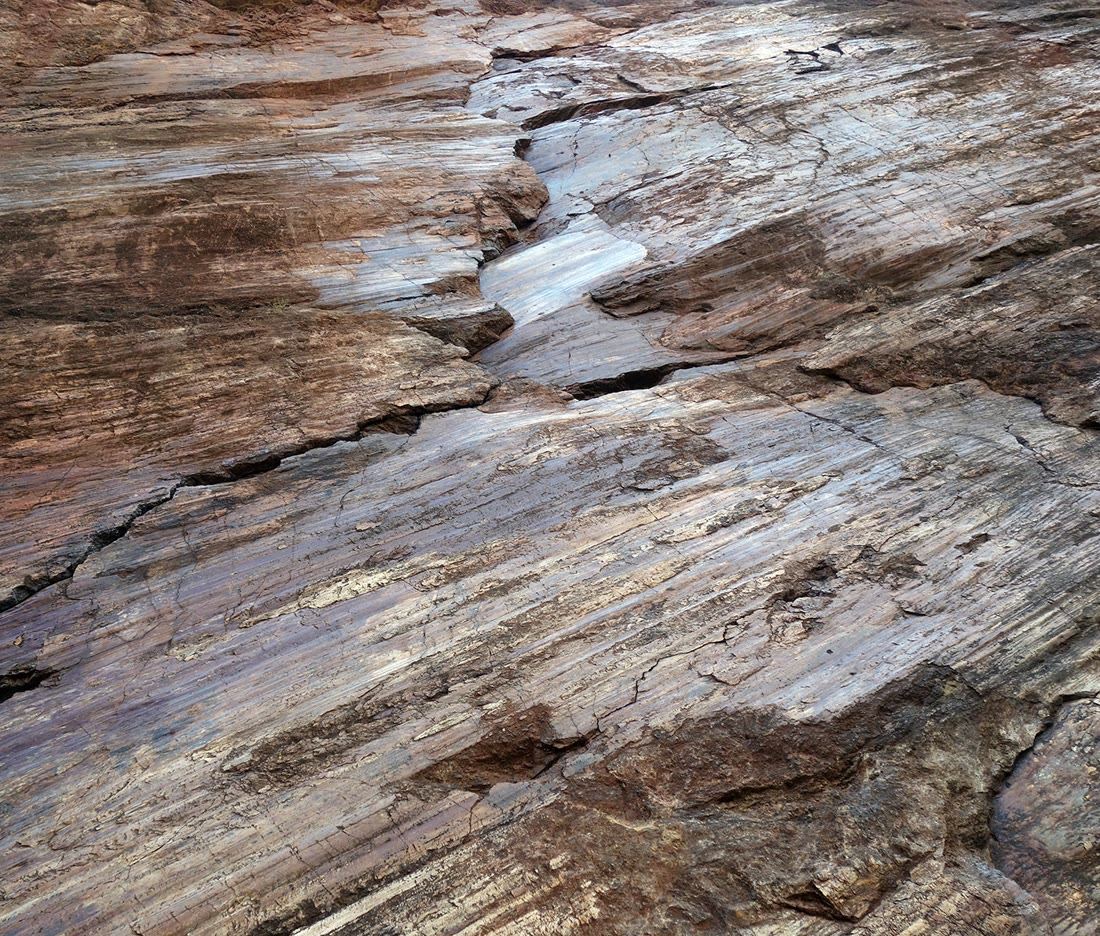
\includegraphics[height=5.2cm]{images/book3/b1-slickenside.jpg}\hfill
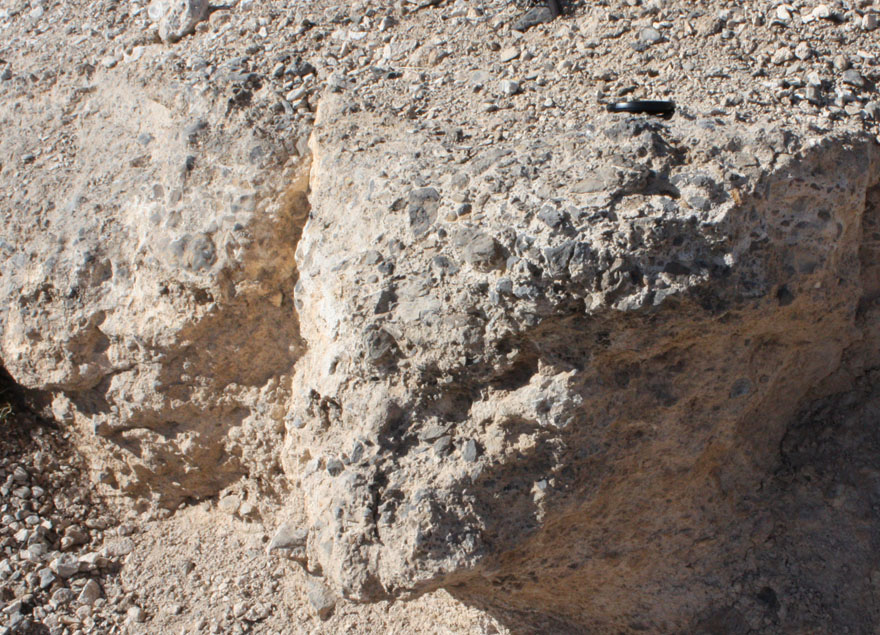
\includegraphics[height=5.2cm]{images/book3/b1-fault-breccia.jpg}
\par\smallskip{\small बाएँ: कोरोना हाइट्स, सैन फ़्रांसिस्को में चर्ट के एक भ्रंश-तल पर एक \omterm{def:b1:faults-folds-fabrics:fault-rocks}{स्लिकेनसाइड}, लगभग \qtyproduct{3 x 3}{m} का, जो \qty{10}{m} ऊँची एक सतह का भाग है; पॉलिश सतह सरकन के अनुदिश धारीदार है। फ़ोटो: Dextersinister, CC~BY-SA~4.0। दाएँ: नेवाडा के रेड रॉक कैन्यन में कीस्टोन थ्रस्ट का \omterm{def:b1:faults-folds-fabrics:fault-rocks}{भ्रंश-ब्रेशिया}: धूसर कार्बोनेट चट्टान के कोणीय टुकड़े एक हल्के आधार में; ऊपर दाईं ओर का लेंस-ढक्कन \qty{5.8}{cm} चौड़ा है। फ़ोटो: Jstuby, सार्वजनिक क्षेत्र। दोनों विकिमीडिया कॉमन्स से।}
\label{fig:b1:faults-folds-fabrics:fault-surfaces}
\end{omfigure}
% ledger: commons:slickenside, commons:breccia

\begin{method}[भ्रंश पर सरकन मापना]\label{met:b1:faults-folds-fabrics:slip}
\begin{enumerate}
  \item भ्रंश-सतह का \omterm{def:b1:geological-maps:attitude}{अभिविन्यास} $\alpha/\delta$ मापिए और उसका \omterm{def:b1:geological-maps:attitude}{स्ट्राइक}, $\alpha - \ang{90}$, लिखिए।
  \item \omterm{def:b1:faults-folds-fabrics:fault-rocks}{स्लिकेनलाइन} मापिए: भ्रंश पर उनका \omterm{def:b1:faults-folds-fabrics:fault-elements}{रेक}, या उनकी दिगंश और अवनति; \omterm{def:b1:faults-folds-fabrics:fault-elements}{रेक} $r$ के लिए, $\sin p = |\sin r|\sin\delta$।
  \item आर-पार विस्थापित चिह्नों से पता लगाइए कि \omterm{def:b1:faults-folds-fabrics:fault-elements}{लटकती दीवार} किस ओर गई, और \omterm{def:b1:faults-folds-fabrics:fault-elements}{रेक} को उसका चिह्न दीजिए: यदि \omterm{def:b1:faults-folds-fabrics:fault-elements}{लटकती दीवार} नीचे गई हो तो ऋणात्मक।
  \item दो ऐसे बिंदुओं से \omterm{def:b1:faults-folds-fabrics:fault-elements}{निवल सरकन} $L$ ज्ञात कीजिए जो कभी एक थे; यदि किसी क्षैतिज चिह्न का केवल भ्रंश का \omterm{def:b1:cross-sections:throw}{विस्थापन} $h$ ज्ञात है, तो $L = h/(|\sin r|\sin\delta)$।
  \item घटक \cref{prop:b1:faults-folds-fabrics:slip-components} से परिकलित कीजिए, और भ्रंश का नाम \cref{def:b1:faults-folds-fabrics:fault-types} से दीजिए।
\end{enumerate}
\end{method}

\begin{inthefield}[भ्रंश-तल का मापन]
एक भूवैज्ञानिक जो उद्भेद में एक भ्रंश-तल पाता है, उसे किसी भी तल की तरह मापता है: एक दिक्सूचक-क्लिनोमीटर उस सतह पर रखकर, और फिर उस पर के \omterm{def:b1:faults-folds-fabrics:fault-rocks}{स्लिकेनलाइन} मापता है, या तो एक प्रोट्रैक्टर से \omterm{def:b1:faults-folds-fabrics:fault-elements}{रेक} के रूप में जो तल पर रखा जाता है, या दिगंश और अवनति के रूप में। दोनों की जाँच विधि के चरण~2 के सूत्र से एक-दूसरे से की जाती है। गति की दिशा तय करना कठिन भाग है। \omterm{def:b1:faults-folds-fabrics:fault-rocks}{स्लिकेनसाइड} पर छोटे सोपान, और क्वार्ट्ज या कैल्साइट के रेशे जो खंडों के दूर जाने के साथ उगे, बता सकते हैं कि लापता खंड किस ओर गया, परंतु कुछ सोपान उलटी दिशा दिखाते हैं, इसलिए दिशा तभी भरोसे की जाती है जब वह किसी चिह्न-परत या शिरा के \omterm{def:b1:cross-sections:throw}{विस्थापन} से मेल खाए। भ्रंश-शैलों का वर्णन और नमूना लिया जाता है, और एक भ्रंश-क्षेत्र जो एक जगह पर मापने के लिए बहुत चौड़ा हो, उसे एक पट्टे के रूप में मानचित्रित किया जाता है। हर भ्रंश को नोटबुक के एक क्रमांकित स्टेशन पर दर्ज किया जाता है, उसके \omterm{def:b1:geological-maps:attitude}{अभिविन्यास}, उसके \omterm{def:b1:faults-folds-fabrics:fault-rocks}{स्लिकेनलाइन}, गति की दिशा और इस बात के साथ कि भूवैज्ञानिक उसके बारे में कितने निश्चित हैं।
\end{inthefield}

\section{एंडरसन का भ्रंश-सिद्धांत}\label{sec:b1:faults-folds-fabrics:anderson}

क्यों अधिकांश \omterm{def:b1:faults-folds-fabrics:fault-types}{सामान्य भ्रंश} खड़े होते हैं और अधिकांश अधिक्षेप मंद? 1905 में स्कॉटिश भूवैज्ञानिक अर्नेस्ट मासन एंडरसन ने दो टिप्पणियों से उत्तर दिया: पृथ्वी की सतह मुख्य प्रतिबलों की दिशाएँ तय करती है, और तब कूलॉम्ब कसौटी भ्रंशों का कोण तय करती है।
% ledger: ws:anderson, anderson:1905

\begin{proposition}[मुक्त सतह एक मुख्य तल बनाती है]\label{prop:b1:faults-folds-fabrics:free-surface}
पृथ्वी की सतह पर, जहाँ वह क्षैतिज है, एक \omterm{def:b1:stress-strain-rheology:principal}{मुख्य प्रतिबल} ऊर्ध्वाधर है और अन्य दो क्षैतिज हैं।
\end{proposition}

\begin{proof}
हवा ज़मीन पर केवल अपने दाब से दबाती है, सतह के लंबवत: वह कोई कर्तन-प्रतिबल नहीं लगाती। इसलिए सतह पर क्षैतिज तल का प्रतिबल उसके लंबवत है।
तीन आयामों में, इकाई अभिलंब $\mathbf n$ वाले तल पर प्रतिबल सदिश $\boldsymbol\sigma\mathbf n$ है (भौतिकी की पुस्तकें); यदि उसका कोई कर्तन भाग नहीं है, तो वह $\mathbf n$ के समांतर है, इसलिए
$\boldsymbol\sigma\mathbf n = \lambda\mathbf n$ और $\mathbf n$ सममित आव्यूह $\boldsymbol\sigma$ का एक अभिलक्षणिक सदिश है: एक मुख्य दिशा (\cref{def:b1:stress-strain-rheology:principal})। अतः ऊर्ध्वाधर एक मुख्य दिशा है, और उसके लंबवत अन्य दो क्षैतिज हैं।
\end{proof}

एंडरसन ने माना कि \omterm{def:b1:stress-strain-rheology:principal}{मुख्य प्रतिबल} इन दिशाओं को उन गहराइयों तक बनाए रखते हैं जिन पर भ्रंश बनते हैं। यह धारणा धीमी ढलान वाली सतह के नीचे और पुराने प्रबल दुर्बलताओं से रहित चट्टानों में ठीक बैठती है; तीव्र उच्चावच के निकट, और जहाँ पुराने भ्रंश या परतें नए भ्रंशों को मार्गदर्शन देती हैं, वह विफल होती है। इसके साथ केवल तीन स्थितियाँ संभव हैं, इस पर निर्भर करते हुए कि $\sigma_1$, $\sigma_2$ और $\sigma_3$ में से कौन ऊर्ध्वाधर है।

\begin{theorem}[एंडरसन का भ्रंश-सिद्धांत]\label{thm:b1:faults-folds-fabrics:anderson}
मान लीजिए एक \omterm{def:b1:stress-strain-rheology:principal}{मुख्य प्रतिबल} ऊर्ध्वाधर है, और चट्टान कूलॉम्ब कसौटी के अनुसार टूटती है, आंतरिक घर्षण कोण $\phi$ के साथ। नए भ्रंश उन तलों पर बनते हैं जिनमें $\sigma_2$ की दिशा है और जो $\ang{45} - \phi/2$ का कोण $\sigma_1$ के साथ बनाते हैं, और वे $\sigma_2$ के लंबवत खिसकते हैं, और चट्टान को $\sigma_1$ के अनुदिश छोटा करते हैं। अतः
\begin{enumerate}[label=(\alph*)]
  \item यदि $\sigma_1$ ऊर्ध्वाधर है, तो \omterm{def:b1:faults-folds-fabrics:fault-types}{सामान्य भ्रंश} बनते हैं, जिनका \omterm{def:b1:geological-maps:attitude}{स्ट्राइक} $\sigma_2$ के अनुदिश हो और जिनकी \omterm{def:b1:geological-maps:attitude}{नति} $\ang{45} + \phi/2$ हो;
  \item यदि $\sigma_3$ ऊर्ध्वाधर है, तो \omterm{def:b1:faults-folds-fabrics:fault-types}{अधिक्षेप भ्रंश} बनते हैं, जिनका \omterm{def:b1:geological-maps:attitude}{स्ट्राइक} $\sigma_2$ के अनुदिश हो और जिनकी \omterm{def:b1:geological-maps:attitude}{नति} $\ang{45} - \phi/2$ हो;
  \item यदि $\sigma_2$ ऊर्ध्वाधर है, तो ऊर्ध्वाधर \omterm{def:b1:faults-folds-fabrics:fault-types}{स्ट्राइक-स्लिप भ्रंश} बनते हैं, जिनका \omterm{def:b1:geological-maps:attitude}{स्ट्राइक} $\ang{45} - \phi/2$ पर, क्षैतिज $\sigma_1$ के दोनों ओर हो।
\end{enumerate}
$\phi = \ang{30}$ के साथ नतियाँ \ang{60}, \ang{30} और \ang{90} हैं।
\end{theorem}
\index{एंडरसन का भ्रंश-सिद्धांत}

\begin{proof}
पहले, जिस तल में $\sigma_2$ की दिशा है, उसका अभिलंब $\sigma_1$ और $\sigma_3$ के तल में है, और तल पर प्रतिबल उस दो-आयामी समस्या का है जो \cref{ch:b1:stress-strain-rheology} में है: उसका बिंदु $\sigma_1$ और $\sigma_3$ के मोर वृत्त पर है, और उसका कर्तन भाग $\sigma_1$ और $\sigma_3$ के तल में, $\sigma_2$ के लंबवत है। किसी अन्य तल पर बिंदु $(\sigma_n, \tau)$ उस वृत्त के भीतर होता है, जो त्रि-आयामी प्रतिबल-अवस्था के तीन मोर वृत्तों में सबसे बड़ा है (त्रि-आयामी सिद्धांत से स्वीकृत)। प्रतिबल बढ़ने पर कूलॉम्ब रेखा इसलिए पहले उन तलों से छुई जाती है जिनमें $\sigma_2$ है, और उनमें से, \cref{thm:b1:stress-strain-rheology:failure-angle} के अनुसार, उन तलों से जो $\ang{45} - \phi/2$ पर $\sigma_1$ से हैं। ऐसे तल पर सरकन, जो $\sigma_2$ के लंबवत है, दोनों खंडों को सबसे अधिक संपीड़न की दिशा में पास लाता है और सबसे कम की दिशा में दूर ले जाता है, जैसा प्रतिबल को राहत देने के लिए होना ही चाहिए। स्थिति (a) में तल ऊर्ध्वाधर से $\ang{45} - \phi/2$ का कोण बनाता है, इसलिए उसकी \omterm{def:b1:geological-maps:attitude}{नति} $\ang{45} + \phi/2$ है; वह क्षैतिज $\sigma_2$ के अनुदिश \omterm{def:b1:geological-maps:attitude}{स्ट्राइक} करता है; सरकन \omterm{def:b1:geological-maps:attitude}{नति} के ऊर्ध्वाधर तल में है, और ऊपर का खंड नीचे जाता है, जिससे चट्टान क्षैतिज रूप से लंबी होती है: एक \omterm{def:b1:faults-folds-fabrics:fault-types}{सामान्य भ्रंश}। स्थिति (b) में तल $\ang{45} - \phi/2 < \ang{45}$ का कोण क्षैतिज $\sigma_1$ के साथ बनाता है, और सरकन चट्टान को क्षैतिज रूप से छोटा करता है, \omterm{def:b1:faults-folds-fabrics:fault-elements}{लटकती दीवार} को ऊपर धकेलते हुए: एक \omterm{def:b1:faults-folds-fabrics:fault-types}{अधिक्षेप भ्रंश}। स्थिति (c) में तल ऊर्ध्वाधर को समाहित करते हैं, इसलिए वे ऊर्ध्वाधर हैं; सरकन क्षैतिज है, $\sigma_2$ के लंबवत: \omterm{def:b1:faults-folds-fabrics:fault-types}{स्ट्राइक-स्लिप भ्रंश}, $\ang{45} - \phi/2$ पर, क्षैतिज $\sigma_1$ के दोनों ओर।
\end{proof}

प्रत्येक शासन में दो समूह भ्रंश संभव हैं, $\sigma_1$ के सममित: संयुग्मी भ्रंश, जो $\ang{90} - \phi$ पर, लगभग \ang{60} पर मिलते हैं, जिनके न्यूनकोण में $\sigma_1$ है। विलोमतः, क्षेत्र में मापे गए एक संयुग्मी भ्रंश युग्म से उन प्रतिबलों की दिशाएँ मिलती हैं जिन्होंने उन्हें बनाया: $\sigma_1$ उनके न्यूनकोण को समद्विभाजित करता है, $\sigma_2$ उनकी प्रतिच्छेद-रेखा है।

\begin{omfigure}
\begin{tikzpicture}[x={(1cm,0cm)}, y={(0.42cm,0.30cm)}, z={(0cm,1cm)},
  >={Stealth[length=5pt]}, font=\small, scale=0.86,
  face/.style={draw=black, line width=0.5pt, line join=round},
  sone/.style={->, line width=1.6pt, omThm},
  sthree/.style={->, line width=0.8pt, omDef}]
% exact geometry: the fault plane is X = xf(Z); slip is along the dip; throw t
% (a) normal fault: dip 60, xf(Z) = 1.3 + (1.6 - Z)/tan 60, throw 0.45
\begin{scope}
  \def\W{3.2}\def\D{1.6}\def\H{1.6}
  \pgfmathsetmacro{\c}{1/tan(60)}
  \pgfmathsetmacro{\xa}{1.3+1.6*\c}       % xf(0)
  \pgfmathsetmacro{\xb}{1.3+0.45*\c}      % xf(H - t)
  \pgfmathsetmacro{\mfa}{1.3+(1.6-0.55)*\c}\pgfmathsetmacro{\mfb}{1.3+(1.6-0.85)*\c}
  \pgfmathsetmacro{\mha}{1.3+(1.6-0.10)*\c}\pgfmathsetmacro{\mhb}{1.3+(1.6-0.40)*\c}
  % footwall
  \fill[omLithSand!55] (0,0,0) -- (\xa,0,0) -- (1.3,0,\H) -- (0,0,\H) -- cycle;
  \fill[omProp!40] (0,0,0.55) -- (\mfa,0,0.55) -- (\mfb,0,0.85) -- (0,0,0.85) -- cycle;
  \draw[face] (0,0,0) -- (\xa,0,0) -- (1.3,0,\H) -- (0,0,\H) -- cycle;
  \draw[face, fill=omLithSand!35] (0,0,\H) -- (1.3,0,\H) -- (1.3,\D,\H) -- (0,\D,\H) -- cycle;
  \draw[face, fill=black!12] (1.3,0,\H) -- (\xb,0,1.15) -- (\xb,\D,1.15) -- (1.3,\D,\H) -- cycle;
  % hanging wall
  \fill[omLithSand!55] (\xa,0,0) -- (\W,0,0) -- (\W,0,1.15) -- (\xb,0,1.15) -- cycle;
  \fill[omProp!40] (\mha,0,0.10) -- (\W,0,0.10) -- (\W,0,0.40) -- (\mhb,0,0.40) -- cycle;
  \draw[face] (\xa,0,0) -- (\W,0,0) -- (\W,0,1.15) -- (\xb,0,1.15) -- cycle;
  \draw[face, fill=omLithSand!35] (\xb,0,1.15) -- (\W,0,1.15) -- (\W,\D,1.15) -- (\xb,\D,1.15) -- cycle;
  \fill[omLithSand!45] (\W,0,0) -- (\W,\D,0) -- (\W,\D,1.15) -- (\W,0,1.15) -- cycle;
  \fill[omProp!30] (\W,0,0.10) -- (\W,\D,0.10) -- (\W,\D,0.40) -- (\W,0,0.40) -- cycle;
  \draw[face] (\W,0,0) -- (\W,\D,0) -- (\W,\D,1.15) -- (\W,0,1.15) -- cycle;
  % slip arrow on the front face
  \draw[->, line width=0.9pt] (1.45,0,1.05) -- ++({0.35*cos(60)},0,{-0.35*sin(60)});
  % stresses: sigma1 vertical, sigma3 horizontal across the strike
  \draw[sone] (1.6,0.8,3.05) -- (1.6,0.8,2.1) node[pos=0, left] {$\sigma_1$};
  \draw[sone] (1.6,0.8,-1.1) -- (1.6,0.8,-0.15);
  \draw[sthree] (-0.85,0.8,0.8) -- (-0.15,0.8,0.8) node[pos=0, above] {$\sigma_3$};
  \draw[sthree] (4.05,0.8,0.6) -- (3.35,0.8,0.6);
  \node[font=\small\bfseries] at (1.9,0,-1.55) {(a) सामान्य भ्रंश};
\end{scope}
% (b) thrust fault: dip 30, xf(Z) = 3.0 - Z/tan 30, throw 0.35, heave 0.606
\begin{scope}[xshift=6.0cm]
  \def\D{1.6}\def\H{1.3}
  \pgfmathsetmacro{\c}{1/tan(30)}
  \pgfmathsetmacro{\Wp}{4.0-0.35*\c}       % right face of the hanging wall
  \pgfmathsetmacro{\xt}{3.0-1.3*\c}        % footwall top edge
  \pgfmathsetmacro{\xh}{3.0-1.65*\c}       % hanging-wall top edge
  \pgfmathsetmacro{\mfa}{3.0-0.50*\c}\pgfmathsetmacro{\mfb}{3.0-0.75*\c}
  \pgfmathsetmacro{\mha}{3.0-0.85*\c}\pgfmathsetmacro{\mhb}{3.0-1.10*\c}
  % footwall
  \fill[omLithSand!55] (0,0,0) -- (3.0,0,0) -- (\xt,0,\H) -- (0,0,\H) -- cycle;
  \fill[omProp!40] (0,0,0.50) -- (\mfa,0,0.50) -- (\mfb,0,0.75) -- (0,0,0.75) -- cycle;
  \draw[face] (0,0,0) -- (3.0,0,0) -- (\xt,0,\H) -- (0,0,\H) -- cycle;
  \draw[face, fill=omLithSand!35] (0,0,\H) -- (\xt,0,\H) -- (\xt,\D,\H) -- (0,\D,\H) -- cycle;
  % hanging wall
  \fill[omLithSand!55] (3.0,0,0) -- (\Wp,0,0) -- (\Wp,0,1.65) -- (\xh,0,1.65) -- cycle;
  \fill[omProp!40] (\mha,0,0.85) -- (\Wp,0,0.85) -- (\Wp,0,1.10) -- (\mhb,0,1.10) -- cycle;
  \draw[face] (3.0,0,0) -- (\Wp,0,0) -- (\Wp,0,1.65) -- (\xh,0,1.65) -- cycle;
  \draw[face, fill=omLithSand!35] (\xh,0,1.65) -- (\Wp,0,1.65) -- (\Wp,\D,1.65) -- (\xh,\D,1.65) -- cycle;
  \fill[omLithSand!45] (\Wp,0,0) -- (\Wp,\D,0) -- (\Wp,\D,1.65) -- (\Wp,0,1.65) -- cycle;
  \fill[omProp!30] (\Wp,0,0.85) -- (\Wp,\D,0.85) -- (\Wp,\D,1.10) -- (\Wp,0,1.10) -- cycle;
  \draw[face] (\Wp,0,0) -- (\Wp,\D,0) -- (\Wp,\D,1.65) -- (\Wp,0,1.65) -- cycle;
  \draw[->, line width=0.9pt] (2.25,0,0.62) -- ++({-0.42*cos(30)},0,{0.42*sin(30)});
  % stresses: sigma1 horizontal across the strike, sigma3 vertical
  \draw[sone] (-1.2,0.8,0.65) -- (-0.15,0.8,0.65) node[pos=0, above] {$\sigma_1$};
  \draw[sone] (\Wp+1.15,0.8,0.45) -- (\Wp+0.1,0.8,0.45);
  \draw[sthree] (2.0,0.8,2.7) -- (2.0,0.8,2.0) node[pos=0, left] {$\sigma_3$};
  \draw[sthree] (2.0,0.8,-0.9) -- (2.0,0.8,-0.2);
  \node[font=\small\bfseries] at (2.0,0,-1.55) {(b) अधिक्षेप भ्रंश};
\end{scope}
% (c) strike-slip fault: vertical, along the y axis at X = 1.6; dextral: the far
% (east) block has moved toward the reader by 0.5; sigma1 at 30 deg clockwise of the strike
\begin{scope}[xshift=12.0cm]
  \def\D{2.2}\def\H{1.1}\def\s{0.5}
  % west block
  \draw[face, fill=omLithSand!55] (0,0,0) -- (1.6,0,0) -- (1.6,0,\H) -- (0,0,\H) -- cycle;
  \draw[face, fill=omLithSand!35] (0,0,\H) -- (1.6,0,\H) -- (1.6,\D,\H) -- (0,\D,\H) -- cycle;
  \draw[face, fill=black!12] (1.6,\D-\s,0) -- (1.6,\D,0) -- (1.6,\D,\H) -- (1.6,\D-\s,\H) -- cycle;
  \draw[line width=1.4pt, omProp] (0,1.25,\H) -- (1.6,1.25,\H);
  % east block
  \draw[face, fill=omLithSand!55] (1.6,-\s,0) -- (3.2,-\s,0) -- (3.2,-\s,\H) -- (1.6,-\s,\H) -- cycle;
  \draw[face, fill=omLithSand!35] (1.6,-\s,\H) -- (3.2,-\s,\H) -- (3.2,\D-\s,\H) -- (1.6,\D-\s,\H) -- cycle;
  \draw[face, fill=omLithSand!45] (3.2,-\s,0) -- (3.2,\D-\s,0) -- (3.2,\D-\s,\H) -- (3.2,-\s,\H) -- cycle;
  \draw[line width=1.4pt, omProp] (1.6,1.25-\s,\H) -- (3.2,1.25-\s,\H);
  % slip arrows on the top
  \draw[->, line width=0.9pt] (2.05,1.35,\H) -- (2.05,0.35,\H);
  \draw[->, line width=0.9pt] (1.15,0.55,\H) -- (1.15,1.55,\H);
  % stresses in the horizontal plane, drawn at the height of the top surface
  \draw[sone] ({1.6+1.9*sin(30)},{0.8+1.9*cos(30)},\H) -- ({1.6+1.0*sin(30)},{0.8+1.0*cos(30)},\H) node[pos=0, right] {$\sigma_1$};
  \draw[sone] ({1.6-1.9*sin(30)},{0.8-1.9*cos(30)},\H) -- ({1.6-1.0*sin(30)},{0.8-1.0*cos(30)},\H);
  \draw[sthree] ({1.6+2.0*sin(120)},{0.8+2.0*cos(120)},\H) -- ({1.6+1.45*sin(120)},{0.8+1.45*cos(120)},\H) node[pos=0, right] {$\sigma_3$};
  \draw[sthree] ({1.6-2.0*sin(120)},{0.8-2.0*cos(120)},\H) -- ({1.6-1.45*sin(120)},{0.8-1.45*cos(120)},\H);
  \node[font=\small\bfseries] at (1.7,0,-1.55) {(c) स्ट्राइक-स्लिप भ्रंश};
\end{scope}
\end{tikzpicture}
\par\smallskip{\small एंडरसन के तीन शासन, प्रमेय की नतियों के साथ, $\phi = \ang{30}$ के लिए: \ang{60}, \ang{30} और ऊर्ध्वाधर। मोटे लाल तीर: $\sigma_1$; पतले नीले तीर: $\sigma_3$; $\sigma_2$ (a) और (b) में भ्रंशों के \omterm{def:b1:geological-maps:attitude}{स्ट्राइक} के अनुदिश चलता है और (c) में ऊर्ध्वाधर है। एक चिह्न-परत (नारंगी) (a) और (b) में भ्रंश के \omterm{def:b1:cross-sections:throw}{विस्थापन} जितनी खिसकती है; (c) में ज़मीन की एक रेखा क्षैतिज रूप से खिसकती है, और भ्रंश \omterm{def:b1:faults-folds-fabrics:fault-types}{दाएँ-पार्श्वीय} है: किसी भी खंड से देखें, दूसरा दाईं ओर गया है। काले तीर सरकन दिखाते हैं।}
\label{fig:b1:faults-folds-fabrics:anderson}
\end{omfigure}

तीन शासन \omterm{def:b1:layered-earth:layers}{भूपर्पटी} के तीन प्रकार के प्लेट-सीमांत से मेल खाते हैं (\cref{ch:b1:rifts-ridges-margins,ch:b1:active-margins})। जहाँ \omterm{def:b1:layered-earth:lithosphere}{स्थलमंडल} खिंचता है, दरारों और कटकों पर, क्षैतिज प्रतिबल ऊर्ध्वाधर से नीचे गिर जाता है और \omterm{def:b1:faults-folds-fabrics:fault-types}{सामान्य भ्रंश} बनते हैं; जहाँ वह दबाया जाता है, अभिसारी सीमांतों और पर्वत-श्रेणियों में, क्षैतिज प्रतिबल चट्टान के भार से अधिक हो जाता है और अधिक्षेप बनते हैं; रूपांतर भ्रंशों के साथ दो क्षैतिज प्रतिबल ऊर्ध्वाधर के दोनों ओर होते हैं। नतियाँ प्रेक्षणों से मोटे तौर पर मेल खाती हैं: दरारों के \omterm{def:b1:faults-folds-fabrics:fault-types}{सामान्य भ्रंश} सतह के निकट लगभग \ang{60} नत हैं, और अधिक्षेप निम्न-कोण \omterm{def:b1:faults-folds-fabrics:fault-types}{उत्क्रम भ्रंश} हैं। अपवाद सूचनाप्रद हैं। कई \omterm{def:b1:faults-folds-fabrics:fault-types}{सामान्य भ्रंश} गहराई के साथ चपटे हो जाते हैं, और दरारों की कुछ काटें उन्हें कर्तन के लगभग समतल क्षेत्र तक पहुँचते दिखाती हैं: ये निम्न-कोण \omterm{def:b1:faults-folds-fabrics:fault-types}{सामान्य भ्रंश}, या विलगन-भ्रंश, \ang{45} से काफ़ी कम पर \omterm{def:b1:layered-earth:layers}{भूपर्पटी} को काटते हैं। एंडरसन का सिद्धांत इन्हें नए भ्रंशों के रूप में नहीं समझा सकता, और \cref{exo:b1:faults-folds-fabrics:10} दिखाता है कि बायरली का घर्षण भी एंडरसनी प्रतिबलों के अंतर्गत इन्हें नहीं सरका सकता: इन्हें दुर्बल भ्रंश-शैलों, उच्च छिद्र-दाब या घूर्णित प्रतिबलों की आवश्यकता है। एक पहले से मौजूद भ्रंश \omterm{prop:b1:stress-strain-rheology:byerlee}{बायरली नियम} के घर्षण पर सरकता है, $\mu = 0.85$, $\phi = \ang{40.4}$; तब सबसे उपयुक्त दिशा वाले \omterm{def:b1:faults-folds-fabrics:fault-types}{सामान्य भ्रंश} \ang{65.2} नत होते हैं, जैसा \cref{ch:b1:stress-strain-rheology} की समस्या ने पाया था।
% ledger: ws:anderson, usgs:fault-types, byerlee:1975

\begin{history}[एंडरसन के भ्रंश]
स्कॉटिश भूवैज्ञानिक अर्नेस्ट मासन एंडरसन ने तीन प्रकार के भ्रंशों का अपना सिद्धांत 1905 में एक छोटे लेख में प्रकाशित किया, भ्रंशन की गतिकी पर, और उसका पूरा रूप, ब्रिटेन के डाइकों और भ्रंशों पर उसके अनुप्रयोग के साथ, अपनी पुस्तक \emph{The Dynamics of Faulting and Dyke Formation} में दिया। कुछ पत्र और वह पुस्तक आज भी संरचनात्मक भूविज्ञान, भूकंप-विज्ञान और शैल-यांत्रिकी को आकार देते हैं: उनके तीन शासन, सामान्य, अधिक्षेप और स्ट्राइक-स्लिप, \omterm{def:b1:layered-earth:layers}{भूपर्पटी} में प्रतिबल-अवस्थाओं और उनके बनाए भ्रंशों को छाँटने का सामान्य तरीका हैं, और भ्रंशों से प्रतिबल पढ़ने का भी।
\end{history}
% ledger: anderson:1905, healy:anderson, ws:anderson

\section{वलन की ज्यामिति}\label{sec:b1:faults-folds-fabrics:folds}

\Cref{ch:b1:geological-maps} ने वलनों को नाम दिए और मानचित्रों पर उनके प्रतिरूप पढ़े। त्रि-आयामी रूप में \omterm{def:b1:geological-maps:fold}{वलन} को और नाम चाहिए: वह कहाँ मुड़ता है, कितनी तीखी मुड़ता है, और अंतरिक्ष में वह कैसे स्थित है।

\begin{definition}[वलन-मोड़, मोड़-रेखा, पार्श्व, अक्षीय तल, अंतर-पार्श्व कोण, बेलनाकार वलन]
\label{def:b1:faults-folds-fabrics:fold-elements}
एक मुड़ी हुई सतह पर, \emph{वलन-मोड़}\index{वलन-मोड़ (वलन का)} वह क्षेत्र है जहाँ वक्रता सबसे अधिक है, और \emph{मोड़-रेखा}\index{मोड़-रेखा} वह रेखा है जो उसके सबसे अधिक वक्रता वाले बिंदुओं को जोड़ती है; \emph{पार्श्व}\index{पार्श्व (वलन का)} दोनों ओर के कम मुड़े हुए भाग हैं। \omterm{def:b1:geological-maps:fold}{वलन} का अक्षीय पृष्ठ वह पृष्ठ है जो उसकी उत्तरोत्तर मुड़ी सतहों की मोड़-रेखाओं को जोड़ता है; जब वह एक तल हो, तो वह \emph{अक्षीय तल}\index{अक्षीय तल} है। \emph{अंतर-पार्श्व कोण}\index{अंतर-पार्श्व कोण} $\iota$ दोनों पार्श्वों के बीच का कोण है, परिच्छेद में मापा गया, मोड़-रेखा के लंबवत तल में, उन स्पर्श-रेखाओं के बीच जो पार्श्वों को उनके नति-परिवर्तन बिंदुओं पर छूती हैं; $0 \le \iota \le \ang{180}$। एक \omterm{def:b1:geological-maps:fold}{वलन} \emph{बेलनाकार वलन}\index{बेलनाकार वलन} है जब उसकी सतहें एक सीधी रेखा को अपने समांतर चलाने से उत्पन्न होती हैं; उस रेखा की दिशा \cref{def:b1:geological-maps:fold} का \omterm{def:b1:geological-maps:fold}{वलन-अक्ष} है, और बेलनाकार \omterm{def:b1:geological-maps:fold}{वलन} की हर मोड़-रेखा उसके समांतर एक सीधी रेखा है।
\end{definition}
% ledger: ws:fold-elements

\begin{omfigure}
\begin{tikzpicture}[x={(1cm,0cm)}, y={(0.42cm,0.30cm)}, z={(0cm,1cm)},
  >={Stealth[length=5pt]}, font=\small, scale=1.15]
% a cylindrical anticline: the top of a bed is z = f(x) = 0.35 a - a sqrt(x^2 + 0.35^2), a = tan 50
% (limbs dip toward 50 deg, interlimb angle 80 deg); the bed is 0.7 thick, measured vertically
% (a similar fold); the fold axis is the y direction, horizontal.
\def\D{2.8}
\pgfmathsetmacro{\a}{tan(50)}
\def\f(#1){0.35*\a - \a*sqrt((#1)*(#1) + 0.1225)}
\pgfmathsetmacro{\zt}{0.35*\a}
% top surface of the bed
\fill[omLithSand!35] plot[domain=-1.7:1.7, samples=61, variable=\x] (\x, 0, {\f(\x)})
  -- plot[domain=1.7:-1.7, samples=61, variable=\x] (\x, \D, {\f(\x)}) -- cycle;
\foreach \u in {-1.4,-1.0,-0.6,-0.3,0.3,0.6,1.0,1.4} {
  \draw[black!35, line width=0.3pt] (\u, 0, {\f(\u)}) -- (\u, \D, {\f(\u)});
}
\draw[line width=0.5pt] plot[domain=-1.7:1.7, samples=61, variable=\x] (\x, \D, {\f(\x)});
\draw[line width=0.5pt] (-1.7, 0, {\f(-1.7)}) -- (-1.7, \D, {\f(-1.7)});
% right end face
\fill[omLithSand!55] (1.7, 0, {\f(1.7)}) -- (1.7, \D, {\f(1.7)}) -- (1.7, \D, {\f(1.7)-0.7}) -- (1.7, 0, {\f(1.7)-0.7}) -- cycle;
\draw[line width=0.5pt] (1.7, 0, {\f(1.7)}) -- (1.7, \D, {\f(1.7)}) -- (1.7, \D, {\f(1.7)-0.7}) -- (1.7, 0, {\f(1.7)-0.7});
% axial plane, behind the front face
\fill[omDef!30, opacity=0.5] (0, 0, 0.85) -- (0, \D, 0.85) -- (0, \D, -2.0) -- (0, 0, -2.0) -- cycle;
\draw[omDef, line width=0.6pt] (0, 0, -2.0) -- (0, 0, 0.85) -- (0, \D, 0.85) -- (0, \D, -2.0);
% hinge line
\draw[omThm, line width=1.5pt] (0, 0, 0) -- (0, \D, 0);
% front face of the bed (the profile)
\fill[omLithSand!80] plot[domain=-1.7:1.7, samples=61, variable=\x] (\x, 0, {\f(\x)})
  -- plot[domain=1.7:-1.7, samples=61, variable=\x] (\x, 0, {\f(\x)-0.7}) -- cycle;
\draw[line width=0.7pt] plot[domain=-1.7:1.7, samples=61, variable=\x] (\x, 0, {\f(\x)});
\draw[line width=0.7pt] plot[domain=-1.7:1.7, samples=61, variable=\x] (\x, 0, {\f(\x)-0.7});
\draw[line width=0.5pt] (-1.7, 0, {\f(-1.7)}) -- (-1.7, 0, {\f(-1.7)-0.7});
\draw[omDef, line width=0.6pt, dashed] (0, 0, 0) -- (0, 0, -0.7);
\draw[omDef, line width=0.6pt] (0, 0, -0.7) -- (0, 0, -2.0);
% interlimb angle on the profile, in the core: tangents to the limbs of the base of the bed
% meet at (0, 0, zt - 0.7)
\pgfmathsetmacro{\zb}{\zt-0.7}
\draw[black!70, dashed] (-1.3, 0, {\zb-1.3*\a}) -- (0, 0, \zb) -- (1.3, 0, {\zb-1.3*\a});
\draw[black, line width=0.5pt] plot[domain=-140:-40, samples=21, variable=\t] ({0.75*cos(\t)}, 0, {\zb+0.75*sin(\t)});
\node[font=\scriptsize] at (0.22, 0, {\zb-1.0}) {$\iota$};
% labels
\node[omThm, anchor=west, font=\scriptsize] at (0.08, \D, 0.1) {मोड़-रेखा};
\node[omDef, anchor=south, font=\scriptsize] at (0, \D, 0.85) {अक्षीय तल};
\node[font=\scriptsize, rotate=50] at (-1.15, 0, {\f(-1.15)-0.35}) {पार्श्व};
\node[font=\scriptsize, rotate=-50] at (1.15, 0, {\f(1.15)-0.35}) {पार्श्व};
\end{tikzpicture}
\par\smallskip{\small एक बेलनाकार \omterm{def:b1:geological-maps:fold}{अपनति}, यहाँ क्षैतिज \omterm{def:b1:faults-folds-fabrics:fold-elements}{मोड़-रेखा} के साथ: मोड़-बिंदु, जहाँ परत सबसे अधिक मुड़ती है; दो \omterm{def:b1:faults-folds-fabrics:fold-elements}{पार्श्व}; \omterm{def:b1:faults-folds-fabrics:fold-elements}{अक्षीय तल}, परत के शीर्ष और आधार की मोड़-रेखाओं से होकर गुज़रता हुआ; और \omterm{def:b1:faults-folds-fabrics:fold-elements}{अंतर-पार्श्व कोण} $\iota$, पार्श्वों की स्पर्श-रेखाओं के बीच, सामने की परिच्छेद में मापा गया, यहाँ \ang{80}, जो परत के आधार पर खींचा गया है। परत के शीर्ष पर धूसर रेखाएँ \omterm{def:b1:geological-maps:fold}{वलन-अक्ष} के समांतर हैं।}
\label{fig:b1:faults-folds-fabrics:fold-elements}
\end{omfigure}

जब \omterm{def:b1:faults-folds-fabrics:fold-elements}{पार्श्व} तल होते हैं, जैसे नीचे के शेवरॉन वलनों में और वार्डन हिल्स में, \omterm{def:b1:geological-maps:fold}{वलन} की ज्यामिति उसके पार्श्वों के \omterm{def:b1:geological-maps:attitude}{अभिविन्यास} से निकलती है। \omterm{def:b1:geological-maps:attitude}{नति-दिशा} $\alpha$ और \omterm{def:b1:geological-maps:attitude}{नति} $\delta$ वाले तल का ऊपर की ओर का इकाई अभिलंब
$\mathbf n = (\sin\delta\sin\alpha, \sin\delta\cos\alpha, \cos\delta)$ है, पूर्व, उत्तर और ऊपर के घटकों में।

\begin{proposition}[वलन उसके पार्श्वों से]\label{prop:b1:faults-folds-fabrics:hinge}
मान लीजिए एक \omterm{def:b1:faults-folds-fabrics:fold-elements}{बेलनाकार वलन} के \omterm{def:b1:faults-folds-fabrics:fold-elements}{पार्श्व} तल हैं, न उलटे हुए, ऊपर की ओर इकाई अभिलंब $\mathbf n_1$ और $\mathbf n_2$ के साथ। उसकी \omterm{def:b1:faults-folds-fabrics:fold-elements}{मोड़-रेखा} $\mathbf n_1 \times \mathbf n_2$ के समांतर है, और उसका \omterm{def:b1:faults-folds-fabrics:fold-elements}{अंतर-पार्श्व कोण}
\[
  \iota = \ang{180} - \arccos(\mathbf n_1\cdot\mathbf n_2) .
\]
\end{proposition}

\begin{proof}
हर \omterm{def:b1:faults-folds-fabrics:fold-elements}{पार्श्व} उस \omterm{def:b1:geological-maps:fold}{वलन-अक्ष} के समांतर रेखाओं से उत्पन्न होता है, इसलिए उसमें अक्ष की दिशा है; अतः वह दिशा दोनों अभिलंबों के लंबवत और उनके सदिश-गुणनफल के समांतर है; \omterm{def:b1:faults-folds-fabrics:fold-elements}{मोड़-रेखा} अक्ष के समांतर है। परिच्छेद अक्ष के लंबवत है, इसलिए उसमें दोनों अभिलंब हैं; उसमें दोनों \omterm{def:b1:faults-folds-fabrics:fold-elements}{पार्श्व} दो रेखाओं के रूप में दिखते हैं, जो $\mathbf n_1$ और $\mathbf n_2$ के लंबवत हैं, और रेखाओं के बीच का कोण अभिलंबों के बीच के कोण $\arccos(\mathbf n_1\cdot\mathbf n_2)$ या उसके संपूरक के बराबर है। जब परतें मुड़ी नहीं होतीं तो दोनों अभिलंब संपाती होते हैं और \omterm{def:b1:faults-folds-fabrics:fold-elements}{अंतर-पार्श्व कोण} \ang{180} होता है; जैसे-जैसे \omterm{def:b1:faults-folds-fabrics:fold-elements}{पार्श्व} घूमते हैं, अभिलंबों के बीच का कोण $0$ से बढ़ता है जबकि \omterm{def:b1:faults-folds-fabrics:fold-elements}{अंतर-पार्श्व कोण} \ang{180} से घटता है, इसलिए दोनों मिलकर \ang{180} होते हैं जब तक दोनों अभिलंब ऊपर की ओर इंगित करते हैं।
\end{proof}

सीधे \omterm{def:b1:geological-maps:fold}{वलन} के लिए, जिसके दोनों \omterm{def:b1:faults-folds-fabrics:fold-elements}{पार्श्व} दोनों ओर $\delta$ नत हैं, अभिलंब कोण $2\delta$ बनाते हैं, और $\iota = \ang{180} - 2\delta$।

\begin{definition}[वलनों के वर्ग]\label{def:b1:faults-folds-fabrics:fold-classes}
\omterm{def:b1:faults-folds-fabrics:fold-elements}{अंतर-पार्श्व कोण} से, एक \omterm{def:b1:geological-maps:fold}{वलन} \emph{मृदु वलन}\index{मृदु वलन} होता है ($\iota$ का मान \ang{180} से \ang{170} तक), एक \emph{खुला वलन}\index{खुला वलन} (\ang{170} से \ang{90} तक), एक \emph{सघन वलन}\index{सघन वलन} (\ang{90} से \ang{10} तक), या, जब उसके \omterm{def:b1:faults-folds-fabrics:fold-elements}{पार्श्व} लगभग समांतर हों ($\iota$ का मान \ang{10} से $0$ तक), एक \emph{समनत वलन}\index{समनत वलन}। \omterm{def:b1:faults-folds-fabrics:fold-elements}{अक्षीय तल} की \omterm{def:b1:geological-maps:attitude}{नति} से, एक \omterm{def:b1:geological-maps:fold}{वलन} \emph{सीधा वलन}\index{सीधा वलन} है जब \omterm{def:b1:faults-folds-fabrics:fold-elements}{अक्षीय तल} \ang{80} से अधिक नत हो, एक \emph{शयित वलन}\index{शयित वलन} जब वह \ang{10} से कम नत हो, और उनके बीच एक \emph{झुका वलन}\index{झुका वलन}। वह \omterm{def:b1:geological-maps:fold}{वलन} जिसका एक \omterm{def:b1:faults-folds-fabrics:fold-elements}{पार्श्व} ऊर्ध्वाधर से आगे मुड़ गया हो, ताकि दोनों \omterm{def:b1:faults-folds-fabrics:fold-elements}{पार्श्व} एक ही ओर नत हों और उस \omterm{def:b1:faults-folds-fabrics:fold-elements}{पार्श्व} की परतें उलटी हों, एक \emph{उलटा वलन}\index{उलटा वलन} है। जिस \omterm{def:b1:geological-maps:fold}{वलन} की \omterm{def:b1:faults-folds-fabrics:fold-elements}{मोड़-रेखा} क्षैतिज न हो, वह एक \emph{अवनत वलन}\index{अवनत वलन} है।
\end{definition}
इस पुस्तक में \omterm{def:b1:geological-maps:fold}{वलन} की कसावट के वर्गों की अन्य सीमाएँ भी प्रयोग में हैं; यह पुस्तक ऊपर के चार रखती है।
% ledger: ws:fold-classes, ws:fold-elements

\begin{omfigure}
\begin{tikzpicture}[font=\small]
% one antiform profile: a hinge arc of radius 0.22 and two straight limbs of length 1.05,
% each at half the interlimb angle (#1 = iota/2) from the downward axial trace; three
% surfaces repeated by a shift of 0.3 along the axial trace (a similar fold)
\newcommand{\foldprof}[2]{%
  \foreach \k in {0,1,2} {
    \draw[line width=0.7pt, #2]
      ($(0,-0.3*\k)+(180-#1:0.22)+({-1.05*sin(#1)},{-1.05*cos(#1)})$)
      -- ($(0,-0.3*\k)+(180-#1:0.22)$)
      arc[start angle=180-#1, end angle=#1, radius=0.22]
      -- ++({1.05*sin(#1)},{-1.05*cos(#1)});
  }
}
% row 1: tightness (the axial plane vertical)
\foreach \i/\n/\x in {174/मृदु/1.5, 120/खुला/4.5, 50/सघन/7.5, 0/समनत/10.5} {
  \begin{scope}[xshift=\x cm]
    \pgfmathsetmacro{\b}{\i/2}
    \draw[omDef, dashed, line width=0.5pt] (0,0.45) -- (0,-1.85);
    \foldprof{\b}{black}
    \node[font=\small\bfseries] at (0,-2.2) {\n};
    \node[font=\scriptsize] at (0,-2.6) {$\iota = \ang{\i}$};
  \end{scope}
}
% row 2: attitude of the axial plane (iota = 40 deg)
\foreach \d/\n/\x in {90/सीधा/1.5, 50/झुका/6.0, 8/शयित/10.5} {
  \begin{scope}[xshift=\x cm, yshift=-4.3cm]
    \begin{scope}[rotate={-(90-\d)}]
      \draw[omDef, dashed, line width=0.5pt] (0,0.55) -- (0,-1.85);
      \foldprof{20}{black}
    \end{scope}
    \node[font=\small\bfseries] at (0,-2.2) {\n};
    \node[font=\scriptsize] at (0,-2.6) {अक्षीय तल की नति \ang{\d}};
  \end{scope}
}
\end{tikzpicture}
\par\smallskip{\small वलनों के वर्ग, परिच्छेद में। ऊपर: \omterm{def:b1:faults-folds-fabrics:fold-elements}{अंतर-पार्श्व कोण} के अनुसार, \omterm{def:b1:faults-folds-fabrics:fold-elements}{अक्षीय तल} ऊर्ध्वाधर (बिंदुकित)। नीचे: \omterm{def:b1:faults-folds-fabrics:fold-elements}{अक्षीय तल} की \omterm{def:b1:geological-maps:attitude}{नति} के अनुसार, \ang{40} \omterm{def:b1:faults-folds-fabrics:fold-elements}{अंतर-पार्श्व कोण} वाले वलनों के लिए; खींचा गया \omterm{def:b1:faults-folds-fabrics:fold-classes}{झुका वलन} उलटा भी है, उसके दोनों \omterm{def:b1:faults-folds-fabrics:fold-elements}{पार्श्व} बाईं ओर नत हैं।}
\label{fig:b1:faults-folds-fabrics:classes}
\end{omfigure}

परतों की मोटाई दो शैलियाँ अलग करती है। समांतर, या संकेंद्री, वलनों में हर परत अपनी लंबवत मोटाई बनाए रखती है, जैसे कागज़ की गड्डी मुड़ने पर करती है; ऐसे \omterm{def:b1:geological-maps:fold}{वलन} बहुत दुर्बल परतों के साथ अंतःस्तरित प्रबल परतों के बकलिंग से बनते हैं। समरूप वलनों में हर सतह का एक ही आकार होता है, परतें \omterm{def:b1:faults-folds-fabrics:fold-elements}{अक्षीय तल} के समांतर मोटाई बनाए रखती हैं, और वे पार्श्वों पर पतली तथा मोड़-बिंदुओं पर मोटी होती हैं, जैसा ऊपर की प्रोफ़ाइलों में है; वे तब बनते हैं जब सारी परतें दुर्बल हों, ताकि वे यांत्रिक भूमिका न निभाएँ। शेवरॉन वलनों के \omterm{def:b1:faults-folds-fabrics:fold-elements}{पार्श्व} सीधे होते हैं और मोड़-बिंदु सँकरे, \omterm{def:b1:faults-folds-fabrics:fold-elements}{अंतर-पार्श्व कोण} \ang{60} के निकट; वे प्रबल परतों के समांतर \omterm{def:b1:geological-maps:fold}{वलन} हैं, जो पास-पास रखी होती हैं और मुड़ते समय एक-दूसरे पर फिसलती हैं।
% ledger: ws:fold-elements

\begin{omfigure}
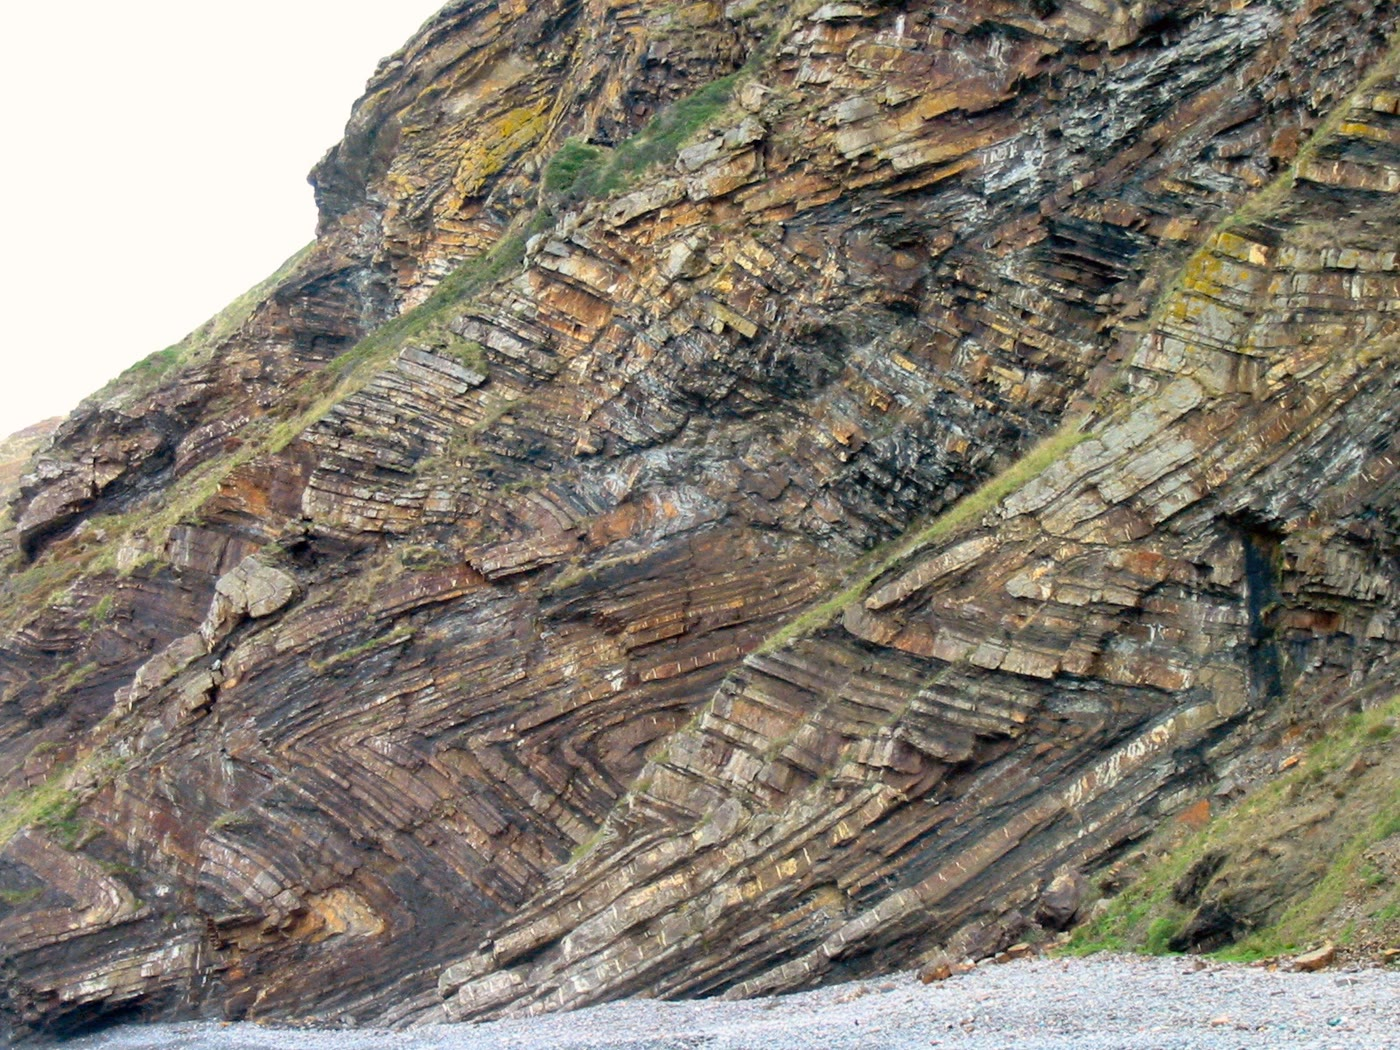
\includegraphics[width=0.78\linewidth]{images/book3/b1-chevron-folds-millook.jpg}
\par\smallskip{\small उत्तरी कॉर्नवॉल में मिलूक की चट्टानों में मुड़ी हुई बलुआ पत्थर और शेल की परतें: शेवरॉन \omterm{def:b1:geological-maps:fold}{वलन}, जिनके लगभग सीधे \omterm{def:b1:faults-folds-fabrics:fold-elements}{पार्श्व} और तीखे मोड़ हैं, और जिनके \omterm{def:b1:faults-folds-fabrics:fold-elements}{अक्षीय तल} लगभग ऊर्ध्वाधर हैं। फ़ोटो: Smalljim, CC~BY~3.0 (विकिमीडिया कॉमन्स)।}
\label{fig:b1:faults-folds-fabrics:chevrons}
\end{omfigure}
% ledger: commons:millook

\section{विन्यास}\label{sec:b1:faults-folds-fabrics:fabrics}

मुड़ी चट्टान अक्सर केवल कुछ सतहों पर नहीं, पूरी तरह विरूपित होती है: उसके कण चपटे, घुमाए या एक साझा दिशा में पुनः उगाए जाते हैं, जो उसे एक विन्यास देता है। समतलीय विन्यास चट्टान को परतों में टूटने देता है, और रैखिक विन्यास उसे छड़ों में टूटने देता है।

\begin{definition}[पर्णन, शिस्टता, स्लेटी विदलन, अक्षीय-तलीय विदलन]\label{def:b1:faults-folds-fabrics:foliation}
\emph{पर्णन}\index{पर्णन} एक समतलीय विन्यास है जो चट्टान में व्याप्त है: अत्यंत पास-पास समांतर सतहों का एक समुच्चय, जो संरेखित पट्टी-जैसे या चपटे कणों से, या पतली परतों से बनता है, और जिसके अनुदिश चट्टान सबसे आसानी से टूटती है। \emph{शिस्टता}\index{शिस्टता} शिस्ट का पर्णन है, जो लगभग \qty{1}{mm} से बड़े संरेखित कणों से बनता है। \emph{विदलन}\index{विदलन (चट्टान का)} एक बारीक-दाना चट्टान का पर्णन है जो उसके विरूपण से बना है; \emph{स्लेटी विदलन}\index{स्लेटी विदलन} स्लेट का विदलन है, जो इतने छोटे \omterm{def:b1:rock-forming-minerals:silicate-classes}{फ़िलोसिलिकेट} खनिजों से बना है कि वे नंगी आँख से नहीं दिखते, और इतने पास-पास रखा हुआ कि चट्टान लगभग कहीं भी पतली चादरों में टूट सकती है। एक \emph{अक्षीय-तलीय विदलन}\index{अक्षीय-तलीय विदलन} वह विदलन है जो उन्हीं चट्टानों में वलनों के अक्षीय तलों के समांतर, या लगभग समांतर है।
\end{definition}
% ledger: ws:fabrics

\omterm{def:b1:faults-folds-fabrics:foliation}{पर्णन} लगभग उस दिशा के लंबवत बनता है जिसमें सबसे अधिक संकुचन है, पट्टी-जैसे कणों के घूमने, नए अभ्रकों के उगने और सबसे जोर से दबाए गए फलकों पर कणों के घुलने से। इसलिए स्लेट का \omterm{def:b1:faults-folds-fabrics:foliation}{विदलन} परतबंदी की मिट्टी से कुछ लेना-देना नहीं रखता: वह दबाव को दर्ज करता है। जब \omterm{def:b1:geological-maps:fold}{वलन} और \omterm{def:b1:faults-folds-fabrics:foliation}{विदलन} एक ही संकुचन में बनते हैं, तो \omterm{def:b1:faults-folds-fabrics:foliation}{विदलन} वलनों के अक्षीय तलों के निकट पड़ता है, और परत की प्रबलता के अनुसार अभिसारी या अपसारी होते हुए, उनके आर-पार हल्का-सा फैलता है, जैसा नीचे का फ़ोटो दिखाता है।
% ledger: ws:fabrics

\begin{omfigure}
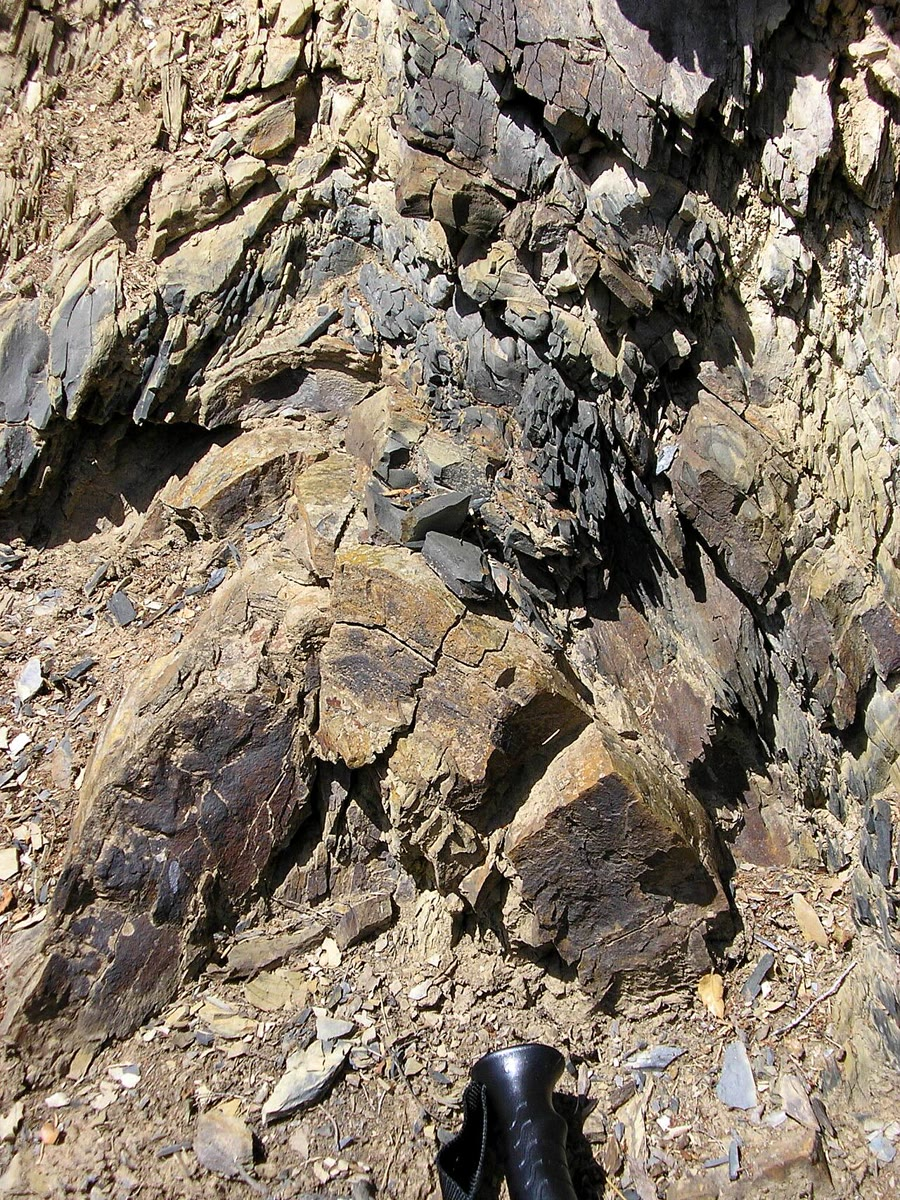
\includegraphics[height=8.2cm]{images/book3/b1-axial-planar-cleavage.jpg}
\par\smallskip{\small स्पेन के कैंटाब्रिया में पोटेस के निकट कार्बोनिफ़ेरस काल के वैकल्पिक बलुआ पत्थर और शेल का एक छोटा \omterm{def:b1:geological-maps:fold}{अपनति}। चित्र के निचले बीच में भूरे बलुआ पत्थर की परतें मोड़-बिंदु पर मेहराब बनाती हैं; उनके ऊपर के गहरे शेल में \omterm{def:b1:faults-folds-fabrics:foliation}{विदलन}, परतों को काटने वाली खड़ी, पास-पास दरारों का समुच्चय, अक्षीय-तलीय है: \omterm{def:b1:geological-maps:fold}{वलन} के \omterm{def:b1:faults-folds-fabrics:fold-elements}{अक्षीय तल} के लगभग समांतर, वह उसके आर-पार फैलता है, और यह फैलाव परत-दर-परत बदलता है। चलने वाली छड़ी का हैंडल लगभग \qty{4}{cm} चौड़ा है। फ़ोटो: Mikenorton, CC~BY-SA~3.0 (विकिमीडिया कॉमन्स)।}
\label{fig:b1:faults-folds-fabrics:cleavage}
\end{omfigure}
% ledger: commons:axial-cleavage

\begin{definition}[रेखन, प्रतिच्छेद-रेखन, खिंचाव-रेखन]\label{def:b1:faults-folds-fabrics:lineation}
\emph{रेखन}\index{रेखन} एक रैखिक विन्यास है जो चट्टान में व्याप्त है, जिसे उसकी दिगंश और अवनति से मापा जाता है। \emph{प्रतिच्छेद-रेखन}\index{प्रतिच्छेद-रेखन} वे रेखाएँ हैं जिनमें दो समतलीय विन्यास एक-दूसरे को काटते हैं, जैसे परतबंदी और \omterm{def:b1:faults-folds-fabrics:foliation}{विदलन}; \emph{खिंचाव-रेखन}\index{खिंचाव-रेखन} वे कण या कंकड़ हैं जो सबसे अधिक खिंचाव की दिशा में खिंचे हुए हैं।
\end{definition}
% ledger: ws:fabrics

\begin{proposition}[एक वलन का प्रतिच्छेद-रेखन]\label{prop:b1:faults-folds-fabrics:intersection}
एक \omterm{def:b1:faults-folds-fabrics:fold-elements}{बेलनाकार वलन} में, जिसमें \omterm{def:b1:faults-folds-fabrics:foliation}{अक्षीय-तलीय विदलन} है, परतबंदी और \omterm{def:b1:faults-folds-fabrics:foliation}{विदलन} का \omterm{def:b1:faults-folds-fabrics:lineation}{प्रतिच्छेद-रेखन} \omterm{def:b1:geological-maps:fold}{वलन} पर हर जगह \omterm{def:b1:faults-folds-fabrics:fold-elements}{मोड़-रेखा} के समांतर है।
\end{proposition}

\begin{proof}
\omterm{def:b1:geological-maps:fold}{वलन} के हर परतीय तल में उसकी अक्ष की दिशा होती है। \omterm{def:b1:faults-folds-fabrics:fold-elements}{अक्षीय तल} में मोड़-रेखाएँ होती हैं, जो अक्ष के समांतर हैं, इसलिए उसमें भी वह दिशा है, और हर \omterm{def:b1:faults-folds-fabrics:foliation}{विदलन} तल भी जो उसके समांतर है। दो तल जो समांतर नहीं हैं और दोनों एक ही दिशा समाहित करते हैं, उस दिशा की एक रेखा पर मिलते हैं।
\end{proof}

यह प्रस्ताव उस \omterm{def:b1:geological-maps:fold}{वलन} की अवनति पाने का क्षेत्र-भूवैज्ञानिक का तरीका है जो एक बार में पूरा दिखाई देने के लिए बहुत बड़ा है: किसी भी \omterm{def:b1:faults-folds-fabrics:fold-elements}{पार्श्व} के किसी भी उद्भेद पर, वे रेखाएँ जिनमें \omterm{def:b1:faults-folds-fabrics:foliation}{विदलन} परतबंदी को काटता है, \omterm{def:b1:faults-folds-fabrics:fold-elements}{मोड़-रेखा} देती हैं। परतबंदी और \omterm{def:b1:faults-folds-fabrics:foliation}{विदलन} मिलकर और भी बताते हैं: \omterm{def:b1:geological-maps:fold}{वलन} कहाँ है, और परतें किस ओर ऊपर हैं।

\begin{definition}[वर्जेंस]\label{def:b1:faults-folds-fabrics:vergence}
असममित \omterm{def:b1:geological-maps:fold}{वलन} का \emph{वर्जेंस}\index{वर्जेंस} वह क्षैतिज दिशा है जिसकी ओर उसका ऊपरी भाग अपने निचले भाग के सापेक्ष चला है: वह दिशा जिसमें वह उलटा है या, झुके \omterm{def:b1:geological-maps:fold}{वलन} के लिए, जिसकी ओर वह झुकता है।
\end{definition}
% ledger: ws:vergence

\begin{proposition}[परतबंदी और विदलन वलन के पार्श्वों पर]\label{prop:b1:faults-folds-fabrics:cleavage-bedding}
मान लीजिए एक \omterm{def:b1:geological-maps:fold}{वलन} है जिसके सीधे \omterm{def:b1:faults-folds-fabrics:fold-elements}{पार्श्व} हैं और एक \omterm{def:b1:faults-folds-fabrics:foliation}{अक्षीय-तलीय विदलन} है, ऐसी चट्टानों में जो मुड़ने से पहले सीधी थीं, और जिनमें दोनों \omterm{def:b1:faults-folds-fabrics:fold-elements}{पार्श्व} हर \omterm{def:b1:geological-maps:fold}{अपनति} के मोड़-बिंदु से नीचे उतरते हैं। परिच्छेद में देखने पर:
\begin{enumerate}[label=(\alph*)]
  \item जिस \omterm{def:b1:faults-folds-fabrics:fold-elements}{पार्श्व} पर परतबंदी और \omterm{def:b1:faults-folds-fabrics:foliation}{विदलन} एक ही ओर नत हैं, परतबंदी दोनों में अधिक खड़ी है ठीक तभी जब वह \omterm{def:b1:faults-folds-fabrics:fold-elements}{पार्श्व} उलटा हो;
  \item \omterm{def:b1:faults-folds-fabrics:foliation}{विदलन} को परतबंदी पर घुमाने वाला न्यूनकोणीय घूर्णन दो पार्श्वों पर विपरीत दिशाओं में होता है; उस \omterm{def:b1:faults-folds-fabrics:fold-elements}{पार्श्व} पर जो उलटा नहीं है, वह \omterm{def:b1:faults-folds-fabrics:foliation}{विदलन} के शीर्ष को क्षैतिज रूप से उस \omterm{def:b1:faults-folds-fabrics:fold-elements}{पार्श्व} के शीर्ष पर अपनति-मोड़ की ओर ले जाता है।
\end{enumerate}
\end{proposition}

\begin{proof}
परिच्छेद में मोड़ के अनुदिश देखिए, जिसमें \omterm{def:b1:faults-folds-fabrics:fold-elements}{अक्षीय तल} बाईं ओर कोण $\gamma$ पर नत है, $0 < \gamma \le \ang{90}$, और क्षैतिज से, दाईं ओर इंगित करते हुए, कोणों को वामावर्त गिनिए। \omterm{def:b1:faults-folds-fabrics:fold-elements}{अक्षीय तल} के समांतर \omterm{def:b1:faults-folds-fabrics:foliation}{विदलन} कोण $\gamma$ पर ऊपर की ओर चलता है। एक \omterm{def:b1:geological-maps:fold}{अपनति} के मोड़ पर दोनों \omterm{def:b1:faults-folds-fabrics:fold-elements}{पार्श्व} नीचे की ओर कोणों $\ang{180} + \gamma - \iota/2$ (\omterm{def:b1:faults-folds-fabrics:fold-elements}{पार्श्व}~1) और $\ang{180} + \gamma + \iota/2$ (\omterm{def:b1:faults-folds-fabrics:fold-elements}{पार्श्व}~2) पर निकलते हैं, \omterm{def:b1:faults-folds-fabrics:fold-elements}{अक्षीय तल} के दोनों ओर, जिसमें $\iota/2 \le \gamma$ है, क्योंकि दोनों नीचे उतरते हैं; वलनों की श्रृंखला का हर \omterm{def:b1:faults-folds-fabrics:fold-elements}{पार्श्व} उस \omterm{def:b1:geological-maps:fold}{अपनति} के लिए इन दोनों में से एक है जो उसके शीर्ष पर है। चट्टानें बाहर की ओर, \omterm{def:b1:geological-maps:fold}{अपनति} के केंद्र से दूर, नई होती जाती हैं, उस \omterm{def:b1:faults-folds-fabrics:fold-elements}{पार्श्व} के अभिलंब के अनुदिश जो \omterm{def:b1:faults-folds-fabrics:fold-elements}{अक्षीय तल} से दूर इंगित करता है।
\omterm{def:b1:faults-folds-fabrics:fold-elements}{पार्श्व}~1 बाईं ओर नीचे जाता है: वह बाईं ओर कोण $\gamma - \iota/2$ पर नत है, \omterm{def:b1:faults-folds-fabrics:foliation}{विदलन} से कम खड़ा। उसका बाहरी अभिलंब, कोण $\ang{90} + \gamma -
\iota/2$ पर, ऊपर की ओर इंगित करता है: वह सीधा है। ऊपर की ओर चलते हुए वह कोण $\gamma - \iota/2$ बनाता है, इसलिए \omterm{def:b1:faults-folds-fabrics:foliation}{विदलन} से परतबंदी तक का न्यूनकोणीय घूर्णन दक्षिणावर्त है, $\iota/2$ से होकर: \omterm{def:b1:faults-folds-fabrics:foliation}{विदलन} का शीर्ष दाईं ओर जाता है, जहाँ मोड़ है, क्योंकि \omterm{def:b1:faults-folds-fabrics:fold-elements}{पार्श्व} मोड़ से बाईं ओर निकलता है।
\omterm{def:b1:faults-folds-fabrics:fold-elements}{पार्श्व}~2 क्षैतिज से ऊपर की ओर कोण $\gamma + \iota/2$ बनाता है। यदि $\gamma + \iota/2 > \ang{90}$ है, तो वह दाईं ओर नीचे जाता है और दाईं ओर नत है, \omterm{def:b1:faults-folds-fabrics:foliation}{विदलन} के विपरीत; उसका बाहरी अभिलंब, कोण $\ang{270} + \gamma +
\iota/2$ पर, ऊपर की ओर का घटक $-\cos(\gamma + \iota/2) > 0$ रखता है: वह सीधा है। यदि $\gamma + \iota/2 < \ang{90}$ है, तो वह बाईं ओर नीचे जाता है, बाईं ओर $\gamma + \iota/2$ पर नत, \omterm{def:b1:faults-folds-fabrics:foliation}{विदलन} से अधिक खड़ा, और वही घटक ऋणात्मक है: \omterm{def:b1:faults-folds-fabrics:fold-elements}{पार्श्व} उलटा है। दोनों स्थितियों में \omterm{def:b1:faults-folds-fabrics:foliation}{विदलन} से परतबंदी तक का न्यूनकोणीय घूर्णन $\iota/2$ से होकर वामावर्त है, और \omterm{def:b1:faults-folds-fabrics:foliation}{विदलन} का शीर्ष बाईं ओर ले जाता है; जब \omterm{def:b1:faults-folds-fabrics:fold-elements}{पार्श्व} सीधा है, तो वह मोड़ से दाईं ओर निकलता है, इसलिए मोड़ बाईं ओर है। \omterm{def:b1:faults-folds-fabrics:foliation}{विदलन} के समान दिशा में नत \omterm{def:b1:faults-folds-fabrics:fold-elements}{पार्श्व} इस प्रकार \omterm{def:b1:faults-folds-fabrics:fold-elements}{पार्श्व}~1 हैं, कम खड़े, और उलटा \omterm{def:b1:faults-folds-fabrics:fold-elements}{पार्श्व}~2, अधिक खड़ा, जो (a) है; घूर्णन \omterm{def:b1:faults-folds-fabrics:fold-elements}{पार्श्व}~1 पर दक्षिणावर्त और \omterm{def:b1:faults-folds-fabrics:fold-elements}{पार्श्व}~2 पर वामावर्त है, जो (b) है।
\end{proof}

मोड़-बिंदु पर, \omterm{def:b1:geological-maps:fold}{अपनति} या \omterm{def:b1:geological-maps:fold}{अभिनति}, घूर्णन की संवेदना बदल जाती है। एक भूवैज्ञानिक जो इसे एक मार्ग पर दर्ज करता है, उन मोड़ों को पाता है जो एक उद्भेद में देखने के लिए बहुत बड़े हैं, जहाँ संवेदना बदलती है, और उलटे पार्श्वों को, जहाँ परतबंदी \omterm{def:b1:faults-folds-fabrics:foliation}{विदलन} से अधिक खड़ी है; घूर्णन की इस संवेदना के लिए शब्द \omterm{def:b1:faults-folds-fabrics:vergence}{वर्जेंस} भी प्रयुक्त होता है, और छोटे वलनों के \omterm{def:b1:faults-folds-fabrics:vergence}{वर्जेंस} के उलटाव उसी प्रकार मानचित्रित किए जाते हैं, ताकि बड़े वलनों के मोड़ मिलें: एक बड़े \omterm{def:b1:geological-maps:fold}{वलन} के दो पार्श्वों के छोटे वलनों की असममिति विपरीत होती है, और उसका अक्षीय अनुरेख उनके बीच से गुज़रता है।
% ledger: ws:vergence, ws:fold-elements

\begin{omfigure}
\begin{tikzpicture}[>={Stealth[length=5pt]}, font=\small]
% a train of chevron folds seen along the hinge (north into the page, east to the right):
% axial planes dipping 60 deg to the west, interlimb angle 40 deg; long limbs dip 40 deg W
% (the right way up), short limbs 80 deg W (overturned). Short limb: from an anticline hinge H_k,
% length s along 260 deg to the syncline hinge S_k; long limb back up along 40 deg to H_{k+1},
% so that all anticline hinges are level, a wavelength w apart.
% Five bedding surfaces, repeated along the axial direction (similar folds); cleavage parallel to it.
\def\s{2.6}
\pgfmathsetmacro{\sx}{\s*cos(260)}\pgfmathsetmacro{\sy}{\s*sin(260)}
\pgfmathsetmacro{\w}{\sx - \sy/tan(40)}
\pgfmathsetmacro{\hx}{0.62*cos(60)}\pgfmathsetmacro{\hy}{0.62*sin(60)}
\newcommand{\surface}[1]{%
  (-\w+#1*\hx, #1*\hy) \foreach \k in {-1,0,1,2,3} { -- ({\k*\w+\sx+#1*\hx}, {\sy+#1*\hy}) -- ({(\k+1)*\w+#1*\hx}, {#1*\hy}) }}
\begin{scope}
  \clip (0.35,-3.3) rectangle (10.0,2.95);
  \begin{scope}
    \clip \surface{0} -- (12,6) -- (-4,6) -- cycle;
    \clip \surface{4} -- (12,-6) -- (-4,-6) -- cycle;
    \fill[omLithSand!45] (-4,-6) rectangle (12,6);
    \fill[omLithShale!40] \surface{2} -- (12,6) -- (-4,6) -- cycle;
    \fill[omLithSand!45] \surface{3} -- (12,6) -- (-4,6) -- cycle;
    \foreach \c in {-8.0,-7.78,...,13.0} {
      \draw[omDef!85, line width=0.35pt] ({\c-6*cot(60)},-6) -- ({\c+6*cot(60)},6);
    }
  \end{scope}
  \foreach \j in {0,1,2,3,4} { \draw[line width=0.75pt, line join=round] \surface{\j}; }
\end{scope}
% axial traces through the anticline hinges, and labels
\foreach \k in {1,2,3} {
  \draw[omThm, dashed, line width=0.6pt] ({\k*\w-0.5*cos(60)},{-0.5*sin(60)}) -- ({\k*\w+3.6*cos(60)},{3.6*sin(60)});
  \node[omThm, font=\scriptsize, anchor=south] at ({\k*\w+3.6*cos(60)},{3.6*sin(60)}) {अपनति};
}
\foreach \k in {1,2,3} { \node[omThm, font=\scriptsize, anchor=north] at ({\k*\w+\sx},{\sy-0.15}) {अभिनति}; }
\end{tikzpicture}
\par\smallskip{\small परिच्छेद में दाईं ओर उलटे शेवरॉन वलनों की एक श्रृंखला, \omterm{def:b1:faults-folds-fabrics:foliation}{अक्षीय-तलीय विदलन} (पतली नीली रेखाएँ) के साथ, पैमाने पर खींची गई: \omterm{def:b1:faults-folds-fabrics:fold-elements}{अक्षीय तल} बाईं ओर \ang{60} नत, \omterm{def:b1:faults-folds-fabrics:fold-elements}{अंतर-पार्श्व कोण} \ang{40}। लंबे \omterm{def:b1:faults-folds-fabrics:fold-elements}{पार्श्व} बाईं ओर \ang{40} नत हैं, \omterm{def:b1:faults-folds-fabrics:foliation}{विदलन} से कम खड़े, और सही क्रम में हैं; छोटे \omterm{def:b1:faults-folds-fabrics:fold-elements}{पार्श्व} बाईं ओर \ang{80} नत हैं, \omterm{def:b1:faults-folds-fabrics:foliation}{विदलन} से अधिक खड़े, और उलटे हैं। \omterm{def:b1:faults-folds-fabrics:foliation}{विदलन} को न्यूनकोण से परतबंदी पर घुमाना हर लंबे \omterm{def:b1:faults-folds-fabrics:fold-elements}{पार्श्व} पर दक्षिणावर्त और हर छोटे \omterm{def:b1:faults-folds-fabrics:fold-elements}{पार्श्व} पर वामावर्त है। इन वलनों का \omterm{def:b1:faults-folds-fabrics:vergence}{वर्जेंस} दाईं ओर है।}
\label{fig:b1:faults-folds-fabrics:vergence}
\end{omfigure}

\section{सूक्ष्म-संरचनाएँ}\label{sec:b1:faults-folds-fabrics:micro}

सूक्ष्मदर्शी के नीचे चट्टान का विरूपण उसके कणों में दिखता है। क्वार्ट्ज का एक कण, जो उसके क्रिस्टल-जालक के धीमे फिसलने से मुड़ा है, क्रॉस्ड पोलरों के बीच एक साथ विलोपन में नहीं जाता: जैसे-जैसे मंच घूमता है, एक गहरी पट्टी उसके आर-पार चलती है, क्योंकि उसके भाग थोड़ी भिन्न दिशाओं में इंगित करते हैं। यह तरंगित विलोपन (\cref{ch:b1:optical-mineralogy}) तब और प्रबल होता है जब कर्तन-क्षेत्र के निकट पहुँचा जाता है, क्योंकि दोष क्रिस्टल-जालक में जमा होते हैं। जहाँ जल है, कण उन फलकों पर घुलते हैं जो सबसे जोर से दबे हैं, और घुला पदार्थ वहाँ जमा होता है जहाँ प्रतिबल कम है, या बह जाता है: यह दाब-विलयन कम ताप पर चट्टानों को छोटा करता है और बहुत-से \omterm{def:b1:faults-folds-fabrics:foliation}{विदलन} बनाता है। अधिक ताप पर विकृत कण, विरूपण जारी रहते हुए, नए, छोटे और अविकृत कणों से बदल जाते हैं, पहले पुरानी कण-सीमाओं के साथ: गतिक पुनर्क्रिस्टलन, जो कण-आकार को सिकोड़ता है और \omterm{def:b1:faults-folds-fabrics:fault-rocks}{मायलोनाइट} बनाता है। विकृत कणों के आकार, और उनकी छायाओं में उगने वाले \omterm{def:b1:rock-forming-minerals:mineral}{खनिज} भी दिखाते हैं कि कर्तन-क्षेत्र किस दिशा में खिसका; ये कर्तन-संवेदना सूचक, और स्वयं ये क्रियाविधियाँ, पुस्तक 5 में हैं।
% ledger: ws:microstructures, ws:fabrics

\section{अभ्यास}

\begin{exercise}[$\star$]
\label{exo:b1:faults-folds-fabrics:1}
हर भ्रंश का नाम उसके \omterm{def:b1:faults-folds-fabrics:fault-elements}{सरकन-सदिश} के \omterm{def:b1:faults-folds-fabrics:fault-elements}{रेक} से दीजिए, वह तल \ang{60} नत है: (a) $r = \ang{-90}$; (b) $r = \ang{85}$; (c) $r = 0$; (d) $r = \ang{180}$; (e) $r = \ang{-40}$। (f) यदि (b) की \omterm{def:b1:geological-maps:attitude}{नति} \ang{25} हो, तो उसे क्या कहेंगे?
% ledger: ar:rake, usgs:fault-types
\end{exercise}

\begin{exercise}[$\star$]
\label{exo:b1:faults-folds-fabrics:2}
एक \omterm{def:b1:faults-folds-fabrics:fault-types}{सामान्य भ्रंश} \ang{55} नत है; उसका सरकन शुद्ध नति-सरकन है, जिसका \omterm{def:b1:faults-folds-fabrics:fault-elements}{निवल सरकन} \qty{300}{m} है। उसका \omterm{def:b1:cross-sections:throw}{विस्थापन} और \omterm{def:b1:cross-sections:throw}{क्षैतिज विस्थापन} परिकलित कीजिए।
\end{exercise}

\begin{exercise}[$\star$]
\label{exo:b1:faults-folds-fabrics:3}
हर ऊर्ध्वाधर \omterm{def:b1:geological-maps:fold}{वलन} का \omterm{def:b1:faults-folds-fabrics:fold-elements}{अंतर-पार्श्व कोण} और वर्ग दीजिए, जिसके \omterm{def:b1:faults-folds-fabrics:fold-elements}{पार्श्व} विपरीत दिशाओं में नत हैं: (a) \omterm{def:b1:faults-folds-fabrics:fold-elements}{पार्श्व} \ang{35} और \ang{35} नत; (b) \ang{70} और \ang{75}; (c) \ang{85} और \ang{88}।
% ledger: ws:fold-classes
\end{exercise}

\begin{exercise}[$\star$]
\label{exo:b1:faults-folds-fabrics:4}
एक बलुआ पत्थर का आंतरिक घर्षण कोण \ang{35} है। एंडरसन के सिद्धांत के अनुसार, उसके \omterm{def:b1:faults-folds-fabrics:fault-types}{सामान्य भ्रंश} और उसके \omterm{def:b1:faults-folds-fabrics:fault-types}{अधिक्षेप भ्रंश} किन कोणों पर नत होते हैं? दो संयुग्मी \omterm{def:b1:faults-folds-fabrics:fault-types}{स्ट्राइक-स्लिप भ्रंश} एक-दूसरे से किस कोण पर बनाते हैं?
\end{exercise}

\begin{exercise}[$\star\star$]
\label{exo:b1:faults-folds-fabrics:5}
एक भ्रंश का \omterm{def:b1:geological-maps:attitude}{अभिविन्यास} $090/50$ है, और उस पर \ang{-30} \omterm{def:b1:faults-folds-fabrics:fault-elements}{रेक} के \omterm{def:b1:faults-folds-fabrics:fault-rocks}{स्लिकेनलाइन} हैं; \omterm{def:b1:faults-folds-fabrics:fault-elements}{निवल सरकन} \qty{400}{m} है। (a) स्ट्राइक-स्लिप और नति-सरकन घटक, भ्रंश का \omterm{def:b1:cross-sections:throw}{विस्थापन} और \omterm{def:b1:cross-sections:throw}{क्षैतिज विस्थापन} परिकलित कीजिए। (b) \omterm{def:b1:faults-folds-fabrics:fault-elements}{सरकन-सदिश} को पूर्व, उत्तर और ऊपर के घटकों में लिखिए, और उसकी दिगंश और अवनति दीजिए। (c) भ्रंश का नाम दीजिए।
\end{exercise}

\begin{exercise}[$\star\star$]
\label{exo:b1:faults-folds-fabrics:6}
दो ऊर्ध्वाधर \omterm{def:b1:faults-folds-fabrics:fault-types}{स्ट्राइक-स्लिप भ्रंश}, एक ही आयु के, $020$ और $080$ \omterm{def:b1:geological-maps:attitude}{स्ट्राइक} करते हैं। (a) एंडरसन के अनुसार $\sigma_1$, $\sigma_2$ और $\sigma_3$ की दिशाएँ, और चट्टान का आंतरिक घर्षण कोण दीजिए। (b) कौन-सा भ्रंश \omterm{def:b1:faults-folds-fabrics:fault-types}{दाएँ-पार्श्वीय} है और कौन-सा \omterm{def:b1:faults-folds-fabrics:fault-types}{बाएँ-पार्श्वीय}? $\sigma_1$ के अनुदिश संकुचन से तर्क दीजिए।
\end{exercise}

\begin{exercise}[$\star\star$]
\label{exo:b1:faults-folds-fabrics:7}
किसी \omterm{def:b1:faults-folds-fabrics:fold-elements}{बेलनाकार वलन} के दो पार्श्वों के \omterm{def:b1:geological-maps:attitude}{अभिविन्यास} $120/40$ और $260/30$ हैं। \cref{prop:b1:faults-folds-fabrics:hinge} से उसकी \omterm{def:b1:faults-folds-fabrics:fold-elements}{मोड़-रेखा} की दिगंश और अवनति, उसका \omterm{def:b1:faults-folds-fabrics:fold-elements}{अंतर-पार्श्व कोण} और उसका वर्ग ज्ञात कीजिए।
\end{exercise}

\begin{exercise}[$\star\star$]
\label{exo:b1:faults-folds-fabrics:8}
एक उद्भेद पर परतबंदी का \omterm{def:b1:geological-maps:attitude}{अभिविन्यास} $040/30$ है और एक \omterm{def:b1:faults-folds-fabrics:foliation}{अक्षीय-तलीय विदलन} का \omterm{def:b1:geological-maps:attitude}{अभिविन्यास} $160/80$। \omterm{def:b1:faults-folds-fabrics:lineation}{प्रतिच्छेद-रेखन} की दिगंश और अवनति ज्ञात कीजिए। वह \omterm{def:b1:geological-maps:fold}{वलन} के बारे में क्या बताती है?
\end{exercise}

\begin{exercise}[$\star\star$]
\label{exo:b1:faults-folds-fabrics:9}
एक ऊर्ध्वाधर भ्रंश पूर्व–पश्चिम \omterm{def:b1:geological-maps:attitude}{स्ट्राइक} करता है। एक ऊर्ध्वाधर डाइक, जो उत्तर–दक्षिण \omterm{def:b1:geological-maps:attitude}{स्ट्राइक} करती है, उसे काटती है; भ्रंश के उत्तर में डाइक, भ्रंश के दक्षिण में जहाँ है उससे \qty{350}{m} पूर्व में पाई जाती है। (a) भ्रंश \omterm{def:b1:faults-folds-fabrics:fault-types}{दाएँ-पार्श्वीय} है या \omterm{def:b1:faults-folds-fabrics:fault-types}{बाएँ-पार्श्वीय}? (b) यदि \omterm{def:b1:faults-folds-fabrics:fault-rocks}{स्लिकेनलाइन} क्षैतिज हैं, तो \omterm{def:b1:faults-folds-fabrics:fault-elements}{निवल सरकन} क्या है? (c) यदि इसके बजाय वे पूर्व की ओर \ang{20} अवनत हैं, तो \omterm{def:b1:faults-folds-fabrics:fault-elements}{निवल सरकन} और सरकन का ऊर्ध्वाधर घटक क्या है, और कौन-सा खंड नीचे गया?
\end{exercise}

\begin{exercise}[$\star\star\star$]
\label{exo:b1:faults-folds-fabrics:10}
संसंजन-रहित और घर्षण गुणांक $\mu$ वाला एक भ्रंश कोण $\theta$ बनाता है $\sigma_1$ के साथ। (a) दिखाइए कि वह तब सरकता है जब प्रभावी \omterm{def:b1:stress-strain-rheology:principal}{मुख्य प्रतिबल} इस अनुपात पर पहुँचें
\[
  \frac{\sigma_1'}{\sigma_3'} = \frac{1 + \mu\cot\theta}{1 - \mu\tan\theta} .
\]
(b) $\mu = 0.6$ और $\sigma_1$ ऊर्ध्वाधर लेकर, \ang{60}, \ang{45} और \ang{35} नत सामान्य भ्रंशों के लिए अनुपात परिकलित कीजिए। (c) दिखाइए कि कोई \omterm{def:b1:faults-folds-fabrics:fault-types}{सामान्य भ्रंश} जो एक निश्चित कोण से कम नत हो, कभी नहीं सरक सकता, और वह कोण परिकलित कीजिए। (d) $\mu = 0.6$ और $\mu = 0.85$ के लिए सबसे उपयुक्त दिशा वाले सामान्य और अधिक्षेप भ्रंशों की नतियाँ दीजिए।
\end{exercise}

\begin{exercise}[$\star\star\star$]
\label{exo:b1:faults-folds-fabrics:11}
पूर्व–पश्चिम के एक मार्ग पर, जिसमें मोड़-रेखाएँ उत्तर की ओर चलती हैं, शेवरॉन वलनों के पार, एक \omterm{def:b1:faults-folds-fabrics:foliation}{अक्षीय-तलीय विदलन} हर जगह पश्चिम की ओर \ang{60} नत है। परतबंदी स्टेशन A पर \ang{40} पश्चिम, स्टेशन B पर \ang{80} पश्चिम और स्टेशन C पर \ang{40} पश्चिम नत है, पश्चिम से पूर्व की ओर, उन चट्टानों में जो मुड़ने से पहले सीधी थीं। (a) कौन-सा स्टेशन उलटे \omterm{def:b1:faults-folds-fabrics:fold-elements}{पार्श्व} पर है? (b) उत्तर की ओर देखते हुए, हर स्टेशन पर \omterm{def:b1:faults-folds-fabrics:foliation}{विदलन} परतबंदी पर किस संवेदना में घूमता है? (c) मोड़ कहाँ हैं, और कौन-से अपनतियाँ हैं? (d) पार्श्वों का \omterm{def:b1:faults-folds-fabrics:fold-elements}{अंतर-पार्श्व कोण} और अक्षीय तलों का \omterm{def:b1:geological-maps:attitude}{अभिविन्यास} ज्ञात कीजिए, और बताइए कि \omterm{def:b1:geological-maps:fold}{वलन} किस ओर झुकते हैं।
\end{exercise}

\begin{exercise}[$\star\star\star$]
\label{exo:b1:faults-folds-fabrics:12}
लंबाई $L_0$ की एक परत एक समरूप शेवरॉन वलनों की श्रृंखला में मुड़ी है, जिसका \omterm{def:b1:faults-folds-fabrics:fold-elements}{अंतर-पार्श्व कोण} $\iota$ है, और उसकी लंबाई अपरिवर्तित है। (a) दिखाइए कि वलनों के आर-पार उसकी मापी गई लंबाई $L_0\sin(\iota/2)$ हो जाती है। (b) \ang{60} \omterm{def:b1:faults-folds-fabrics:fold-elements}{अंतर-पार्श्व कोण} वाले शेवरॉन \omterm{def:b1:geological-maps:fold}{वलन} कितना संकुचन दर्शाते हैं? (c) \qty{30}{\percent} संकुचन के अनुरूप कौन-सा \omterm{def:b1:faults-folds-fabrics:fold-elements}{अंतर-पार्श्व कोण} है? (d) \ang{12} नत पार्श्वों वाली सीधे वलनों की श्रृंखला: कितना संकुचन?
\end{exercise}

\section{समस्या: वार्डन हिल्स की संरचनाएँ, मापी गईं}

\begin{problem}[{सप्ताहांत समस्या --- वार्डन हिल्स की अपनति और सामान्य भ्रंश, तलों की अभिविन्यासों से भ्रंश पर सरकन तक}]
\label{pb:b1:faults-folds-fabrics:1}
% values: calc/ch17.py; region: figdata/shared/region.py (limbs, plunge, fault)
वार्डन हिल्स एक \omterm{def:b1:geological-maps:fold}{अपनति} में मुड़ी हैं, जिसकी धुरी $x = \qty{3.5}{km}$ पर उत्तर–दक्षिण चलती है, और उससे \qty{4}{km} पूर्व में एक \omterm{def:b1:geological-maps:fold}{अभिनति} है; दोनों के \omterm{def:b1:faults-folds-fabrics:fold-elements}{पार्श्व} तल हैं। एक क्षेत्र-सर्वेक्षण ने \omterm{def:b1:geological-maps:fold}{अपनति} के पूर्वी \omterm{def:b1:faults-folds-fabrics:fold-elements}{पार्श्व} पर परतबंदी को $080.7/12.2$ और उसके पश्चिमी \omterm{def:b1:faults-folds-fabrics:fold-elements}{पार्श्व} पर $279.3/12.2$ मापा। आवरण को $120/60$ \omterm{def:b1:geological-maps:attitude}{अभिविन्यास} का एक \omterm{def:b1:faults-folds-fabrics:fault-types}{सामान्य भ्रंश} काटता है, जिसकी \omterm{def:b1:faults-folds-fabrics:fault-elements}{लटकती दीवार} \omterm{def:b1:geological-maps:attitude}{नति} के अनुदिश नीचे गई है, और उसका भ्रंश का \omterm{def:b1:cross-sections:throw}{विस्थापन} \qty{200}{m} है। कोण \ang{0.1} तक और लंबाइयाँ \qty{0.1}{m} तक दीजिए।

\medskip
\noindent\textbf{भाग I --- पार्श्व।}
\begin{enumerate}
  \item ऊपर की ओर के इकाई अभिलंब $\mathbf n_1$ (पूर्वी \omterm{def:b1:faults-folds-fabrics:fold-elements}{पार्श्व}) और $\mathbf n_2$ (पश्चिमी \omterm{def:b1:faults-folds-fabrics:fold-elements}{पार्श्व}) पूर्व, उत्तर और ऊपर के घटकों में लिखिए।
  \item $\mathbf n_1\cdot\mathbf n_2$ और दोनों अभिलंबों के बीच का कोण परिकलित कीजिए।
  \item \omterm{def:b1:geological-maps:fold}{अपनति} का \omterm{def:b1:faults-folds-fabrics:fold-elements}{अंतर-पार्श्व कोण} निकालिए।
  \item \omterm{def:b1:geological-maps:fold}{अपनति} को उसके \omterm{def:b1:faults-folds-fabrics:fold-elements}{अंतर-पार्श्व कोण} से वर्गीकृत कीजिए।
  \item दोनों \omterm{def:b1:faults-folds-fabrics:fold-elements}{पार्श्व} \ang{12.2} नत हैं। \omterm{def:b1:faults-folds-fabrics:fold-elements}{अंतर-पार्श्व कोण} ठीक $\ang{180} - 2\times\ang{12.2}$ क्यों नहीं है? पूर्व–पश्चिम ऊर्ध्वाधर काट में किसी भी \omterm{def:b1:faults-folds-fabrics:fold-elements}{पार्श्व} की \omterm{def:b1:cross-sections:apparent-dip}{आभासी नति} परिकलित कीजिए।
  \item \omterm{def:b1:geological-maps:fold}{अभिनति} \omterm{def:b1:geological-maps:fold}{अपनति} के पूर्वी \omterm{def:b1:faults-folds-fabrics:fold-elements}{पार्श्व} को साझा करती है, और उसका अपना पूर्वी \omterm{def:b1:faults-folds-fabrics:fold-elements}{पार्श्व} \omterm{def:b1:geological-maps:fold}{अपनति} के पश्चिमी \omterm{def:b1:faults-folds-fabrics:fold-elements}{पार्श्व} के समांतर है। उसका \omterm{def:b1:faults-folds-fabrics:fold-elements}{अंतर-पार्श्व कोण} क्या है?
\end{enumerate}

\medskip
\noindent\textbf{भाग II --- मोड़-रेखा और अक्षीय तल।}
\begin{enumerate}[resume]
  \item $\mathbf n_1\times\mathbf n_2$, और \omterm{def:b1:faults-folds-fabrics:fold-elements}{मोड़-रेखा} की दिगंश और अवनति परिकलित कीजिए।
  \item \omterm{def:b1:faults-folds-fabrics:fold-elements}{अक्षीय तल} का \omterm{def:b1:geological-maps:attitude}{अभिविन्यास} दीजिए। क्या \omterm{def:b1:geological-maps:fold}{अपनति} सीधी, झुकी या शयित है?
  \item \omterm{def:b1:geological-maps:fold}{वलन} का पूरा वर्णन दीजिए: कसावट, \omterm{def:b1:faults-folds-fabrics:fold-elements}{अक्षीय तल} का \omterm{def:b1:geological-maps:attitude}{अभिविन्यास}, अवनति।
  \item \cref{ch:b1:geological-maps} के \omterm{def:b1:geological-maps:geological-map}{भूवैज्ञानिक मानचित्र} पर, \omterm{def:b1:geological-maps:fold}{अपनति} के उद्भेद किस ओर बंद होते हैं, और उसके केंद्र में क्या निकलता है?
  \item आवरण का शेल एक \omterm{def:b1:faults-folds-fabrics:foliation}{अक्षीय-तलीय विदलन} रखता है। उसका \omterm{def:b1:geological-maps:attitude}{अभिविन्यास} दीजिए, और पूर्वी \omterm{def:b1:faults-folds-fabrics:fold-elements}{पार्श्व} पर उसके \omterm{def:b1:faults-folds-fabrics:lineation}{प्रतिच्छेद-रेखन} की दिगंश और अवनति दीजिए।
  \item पूर्वी \omterm{def:b1:faults-folds-fabrics:fold-elements}{पार्श्व} पर, उत्तर की ओर देखते हुए, \omterm{def:b1:faults-folds-fabrics:foliation}{विदलन} परतबंदी पर किस संवेदना में घूमता है, और मोड़ किस ओर है?
\end{enumerate}

\medskip
\noindent\textbf{भाग III --- भ्रंश और प्रतिबल।}
\begin{enumerate}[resume]
  \item भ्रंश का \omterm{def:b1:geological-maps:attitude}{स्ट्राइक} दाएँ-हाथ नियम से दीजिए, और बताइए कि \omterm{def:b1:faults-folds-fabrics:fault-elements}{लटकती दीवार} उसके अनुरेख के किस ओर है।
  \item एंडरसन के अनुसार, भ्रंश बनते समय कौन-सा \omterm{def:b1:stress-strain-rheology:principal}{मुख्य प्रतिबल} ऊर्ध्वाधर था?
  \item दोनों क्षैतिज मुख्य प्रतिबलों की दिशाएँ दीजिए।
  \item \omterm{def:b1:geological-maps:attitude}{नति} से कौन-सा आंतरिक घर्षण कोण सूचित होता है? घर्षण गुणांक क्या है?
  \item वे संयुग्मी भ्रंश समुच्चय, जिन्हें वही प्रतिबल बना सकते थे, उनका \omterm{def:b1:geological-maps:attitude}{अभिविन्यास} दीजिए, और दोनों समुच्चयों के बीच का कोण भी।
  \item क्या वही शासन के अंतर्गत यह भ्रंश, 0.85 के बायरली घर्षण के साथ, फिर सरकने के लिए सबसे उपयुक्त दिशा में होगा?
\end{enumerate}

\medskip
\noindent\textbf{भाग IV --- सरकन।}
\begin{enumerate}[resume]
  \item \omterm{def:b1:faults-folds-fabrics:fault-elements}{रेक} और \omterm{def:b1:faults-folds-fabrics:fault-elements}{सरकन-सदिश} की दिगंश और अवनति दीजिए।
  \item \omterm{def:b1:faults-folds-fabrics:fault-elements}{सरकन-सदिश} को पूर्व, उत्तर और ऊपर के घटकों में लिखिए।
  \item भ्रंश का \omterm{def:b1:cross-sections:throw}{क्षैतिज विस्थापन} परिकलित कीजिए।
  \item भ्रंश की \omterm{def:b1:faults-folds-fabrics:fault-elements}{लटकती दीवार} के \omterm{def:b1:cross-sections:throw}{क्षैतिज विस्थापन} के पूर्व और उत्तर घटक परिकलित कीजिए।
  \item जाँच कीजिए कि \omterm{def:b1:faults-folds-fabrics:fault-elements}{निवल सरकन} $L$, भ्रंश का \omterm{def:b1:cross-sections:throw}{विस्थापन} $h$ और \omterm{def:b1:cross-sections:throw}{क्षैतिज विस्थापन} $e$ $L^2 = h^2 + e^2$ को संतुष्ट करते हैं, और समझाइए क्यों।
  \item वार्डन भ्रंश का \omterm{def:b1:faults-folds-fabrics:fault-elements}{निवल सरकन}, निकटतम मीटर तक, क्या है?
\end{enumerate}
\end{problem}
